\pdfminorversion=7
\documentclass[usepdftitle=false,aspectratio=169,xcolor=dvipsnames]{beamer}

\begingroup\expandafter\ifx\csname pdfsuppresswarningpagegroup\endcsname\relax\else\global\pdfsuppresswarningpagegroup=1\relax\fi\endgroup
%\pdfsuppresswarningpagegroup=1 % to suppress warnings of multiple pictures on same page

\usepackage{arydshln}
\usepackage[T1]{fontenc}
\usepackage{threeparttable}
\usepackage{booktabs}
\usepackage{setspace}
%\usepackage{appendixnumberbeamer}
\usepackage{tabularx}

  \usepackage[english]{babel}
  \usepackage[latin1]{inputenc}
  \usepackage{amsmath,amsthm, amssymb,latexsym,bbm}
  \usefonttheme[onlymath]{serif}
%  \boldmath

\usepackage{tikz}

\newtheorem{proposition}{Proposition}


\usetheme{Singapore}
\usecolortheme{seagull}

\definecolor{darkred}{rgb}{0.8,0,.22}
\definecolor{lightgrey}{rgb}{0.855,0.855,0.855}
\definecolor{darkgrey}{rgb}{0.695,0.695,0.695}
\setbeamercolor{alerted text}{fg=darkred!80!black}
\setbeamercolor{structure}{fg=black}
\setbeamercolor{block title}{fg=darkred}
\definecolor{beamer@blendedblue}{rgb}{0.6,0.6,0.6} % use structure theme to change
\setbeamercolor{titlelike}{bg=white,fg=darkred}
\setbeamercolor{frametitle}{bg=white,fg=darkred}
\setbeamercolor*{separation line}{}
\setbeamercolor*{fine separation line}{}


 \setbeamercovered{transparent}
\setbeamertemplate{footline} {\hfill
 \insertframenumber{} / \inserttotalframenumber\mbox{ }\vspace{1mm}%
} \setbeamertemplate{navigation symbols}{}


\mode<presentation>

\parskip3mm


\usepackage{colortbl, xcolor}
\usepackage{graphicx}
\usepackage{subcaption}
\usepackage{pifont,threeparttable}

\newcommand{\cov}{\nu}
\newcommand{\mincov}{\underline{\nu}}
%\newcommand{\common}{\upsilon}

\makeatother



\title{Catholic Censorship and the Demise of Knowledge Production in Early Modern Italy }
\author{Fabio Blasutto\(^{*}\) \and David de la Croix\(^{\dag}\)}
\institute{\(^{*}\)Stockholm School of Economics \quad
\(^{\dag}\)IRES/LIDAM, UCLouvain \& CEPR}
\date{Toulouse, June 2022\\
\vspace{0.5cm}

\includegraphics[width=6cm]{logo-erc.png}}


\begin{document}
	


	\begin{frame}
		\titlepage
	\end{frame}
	
	\section{Introduction}
	\subsection{}
	
	\begin{frame}

\frametitle{The decline of Italy}

15-16th centuries: undisputed Italy's primacy in knowledge creation (Galileo)

 North and Western Europe overtook Italy in the following two centuries

 Reasons for the relative decline of Italy ? Counter-Reformation (Landes 1999) or war \& pandemics (Alfani)

The  Church started to fight against the ideas which will produce the Scientific Revolution

Several tools used. Here focus on \textit{Index Librorum Prohibitorum} - censorship

Could censorship be important for Italy's demise ?

	\end{frame}
	
	\begin{frame}
\frametitle{Censorship}

Key idea
\begin{itemize}
\item Censorship makes new ideas less available to others,
\item distorts people choice to develop non-compliant ideas (occupational choice)
\end{itemize}

Structural approach to model  occupational choice mechanism and assess its weight
\begin{itemize}
\item construct a large sample of academic scholars
active in Italy from 1400 to 1750 and  document  the intensity of censorship,
\item measure their quality (human capital)  through publications
\item  identify the deep parameters of a novel model linking censorship to knowledge diffusion and
occupational choice,
\item  counterfactual experiment to assess quantitatively
the role of censorship in the decline in total publications per scholar in Italy.
\end{itemize}

	\end{frame}

	\begin{frame}
\frametitle{Preview of the results (1)}

New facts
\begin{itemize}
\item in the sixteenth century,  censored authors were of much better quality than  non-censored authors,
\item less and less true as time passes,
\item  intensity of censorship decreased over time.
\end{itemize}

Model
\begin{itemize}
\item  growth model with novel occupational choice made by printers between printing compliant/conformist books or revolutionary/non-conformist books
\end{itemize}

	\end{frame}

	\begin{frame}
\frametitle{Preview of the results (2)}

Quantitative (calibration - simulation)
\begin{itemize}
\item  imposing a censorship rate of 19\% on the non-conformist books was sufficient to decrease the share of non-conformist authors from 51\% in 1470-1550 to 24\% in 1680-1750,
\item  censorship reduced by 40\% the average log publication per scholar in Italy,
\item  half of this drop stems from the induced reallocation of talents towards compliant activities,
\item The effect of adverse macroeconomic conditions on knowledge production is one fourth of  the effect of censorship.
\end{itemize}


	\end{frame}


	\begin{frame}
\frametitle{Literature}

Literature on the effects of censorship in other contexts.  Our innovation: endogenous selection of agents into compliant vs. non-compliant knowledge

Literature on  Catholic censorship,  Becker, Pino, and Vidal-Robert (2021) and
Comino, Galasso, and Graziano (2021). They focus on books. We focus on authors, their quality, and have structural growth model.

Interactions between church and society, B\'enabou, Ticchi, and Vindigni (2021).  We rationalize  the Church's late reaction to the rise of
Protestantism.

Literature on the decline of Italy.


	\end{frame}


	\section{Data}
	\subsection{}

	\begin{frame}
\frametitle{Academies, Scholars, Publications, and Censorship}

Our unit of observation is an academic scholar active in Italy over 1400-1750.

Start from list of universities (Frijhoff) and academies (McClelland, British Library)

Establish list of their members from secondary sources

Look for their publications in Worldcat

Look if they were censored in \textit{Index Librorum Prohibitorum} (Bujanda 2002)

\end{frame}


	\begin{frame}
\frametitle{Example}

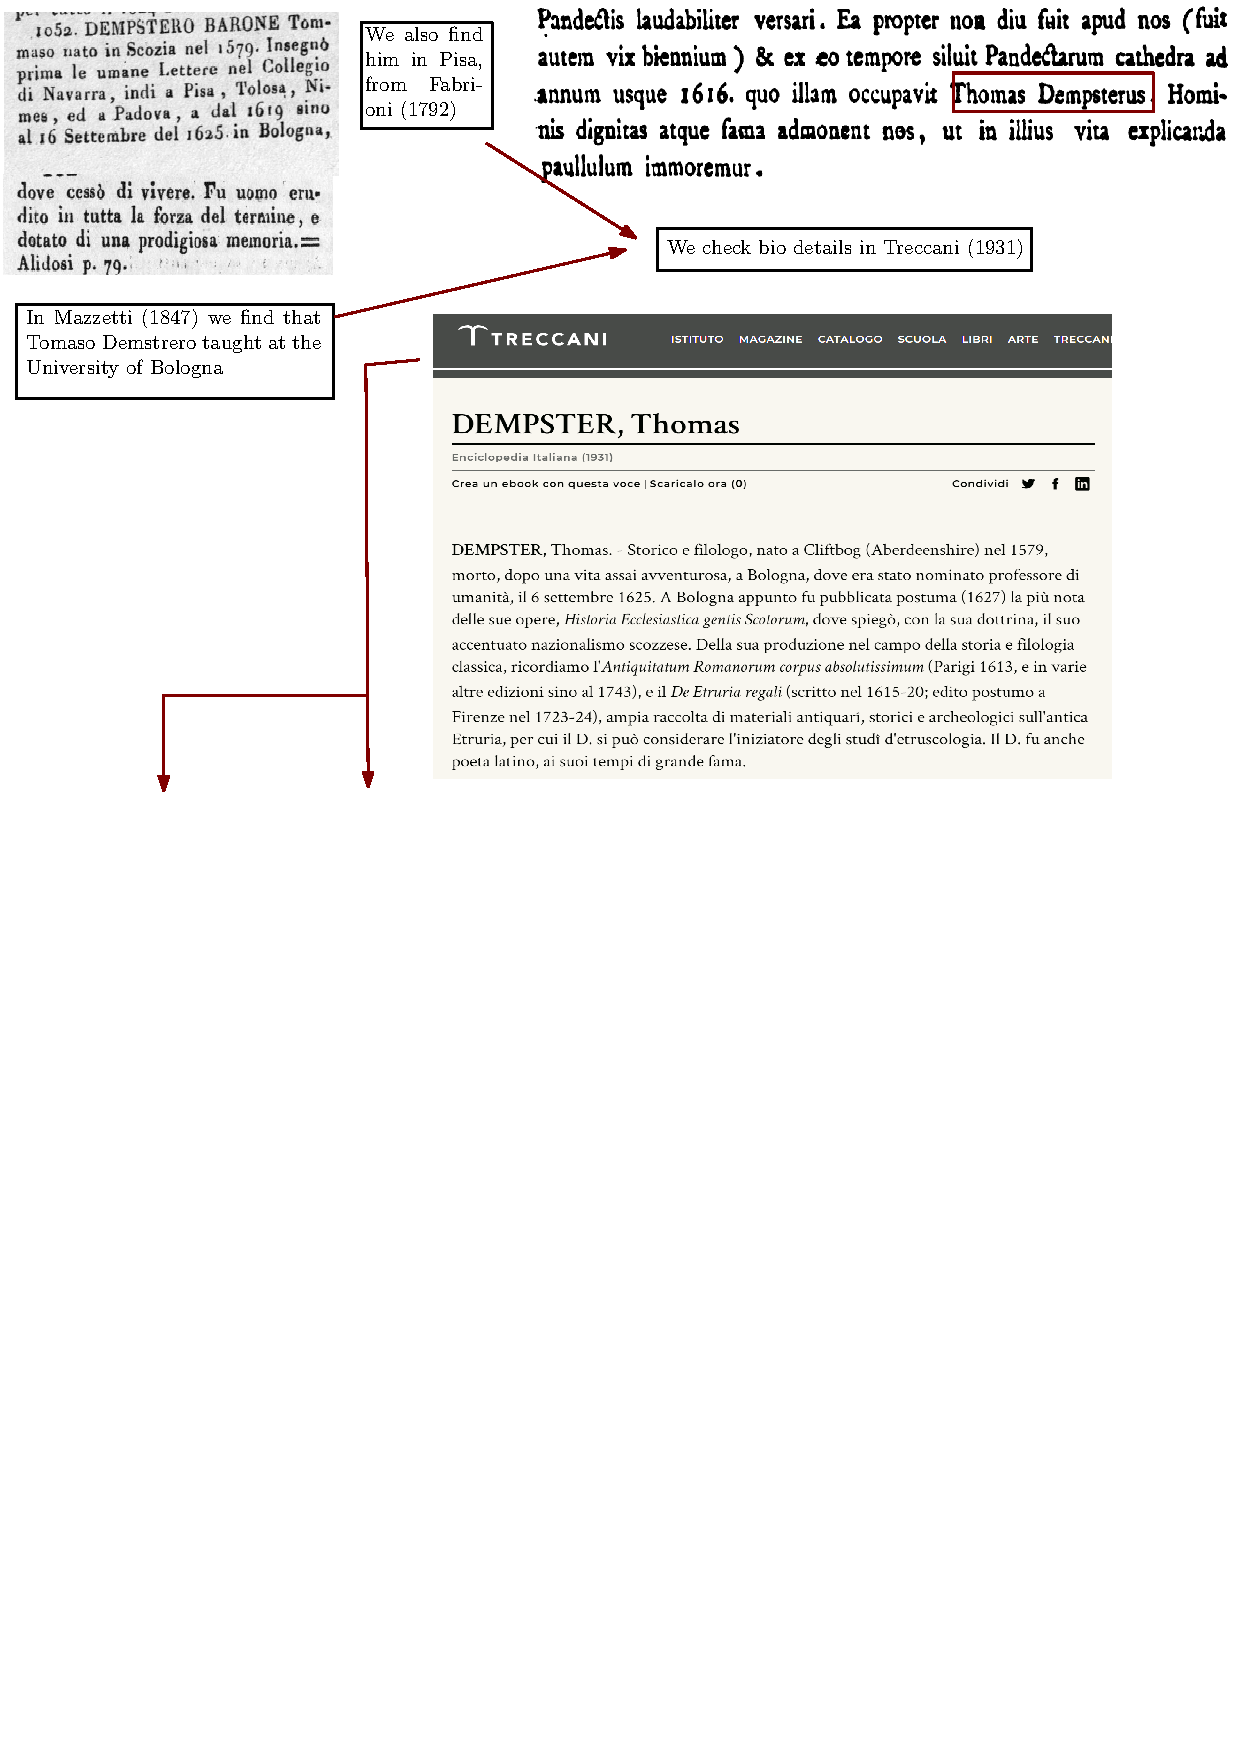
\includegraphics[width=.75\textwidth]{dempster1.pdf}

\end{frame}


	\begin{frame}

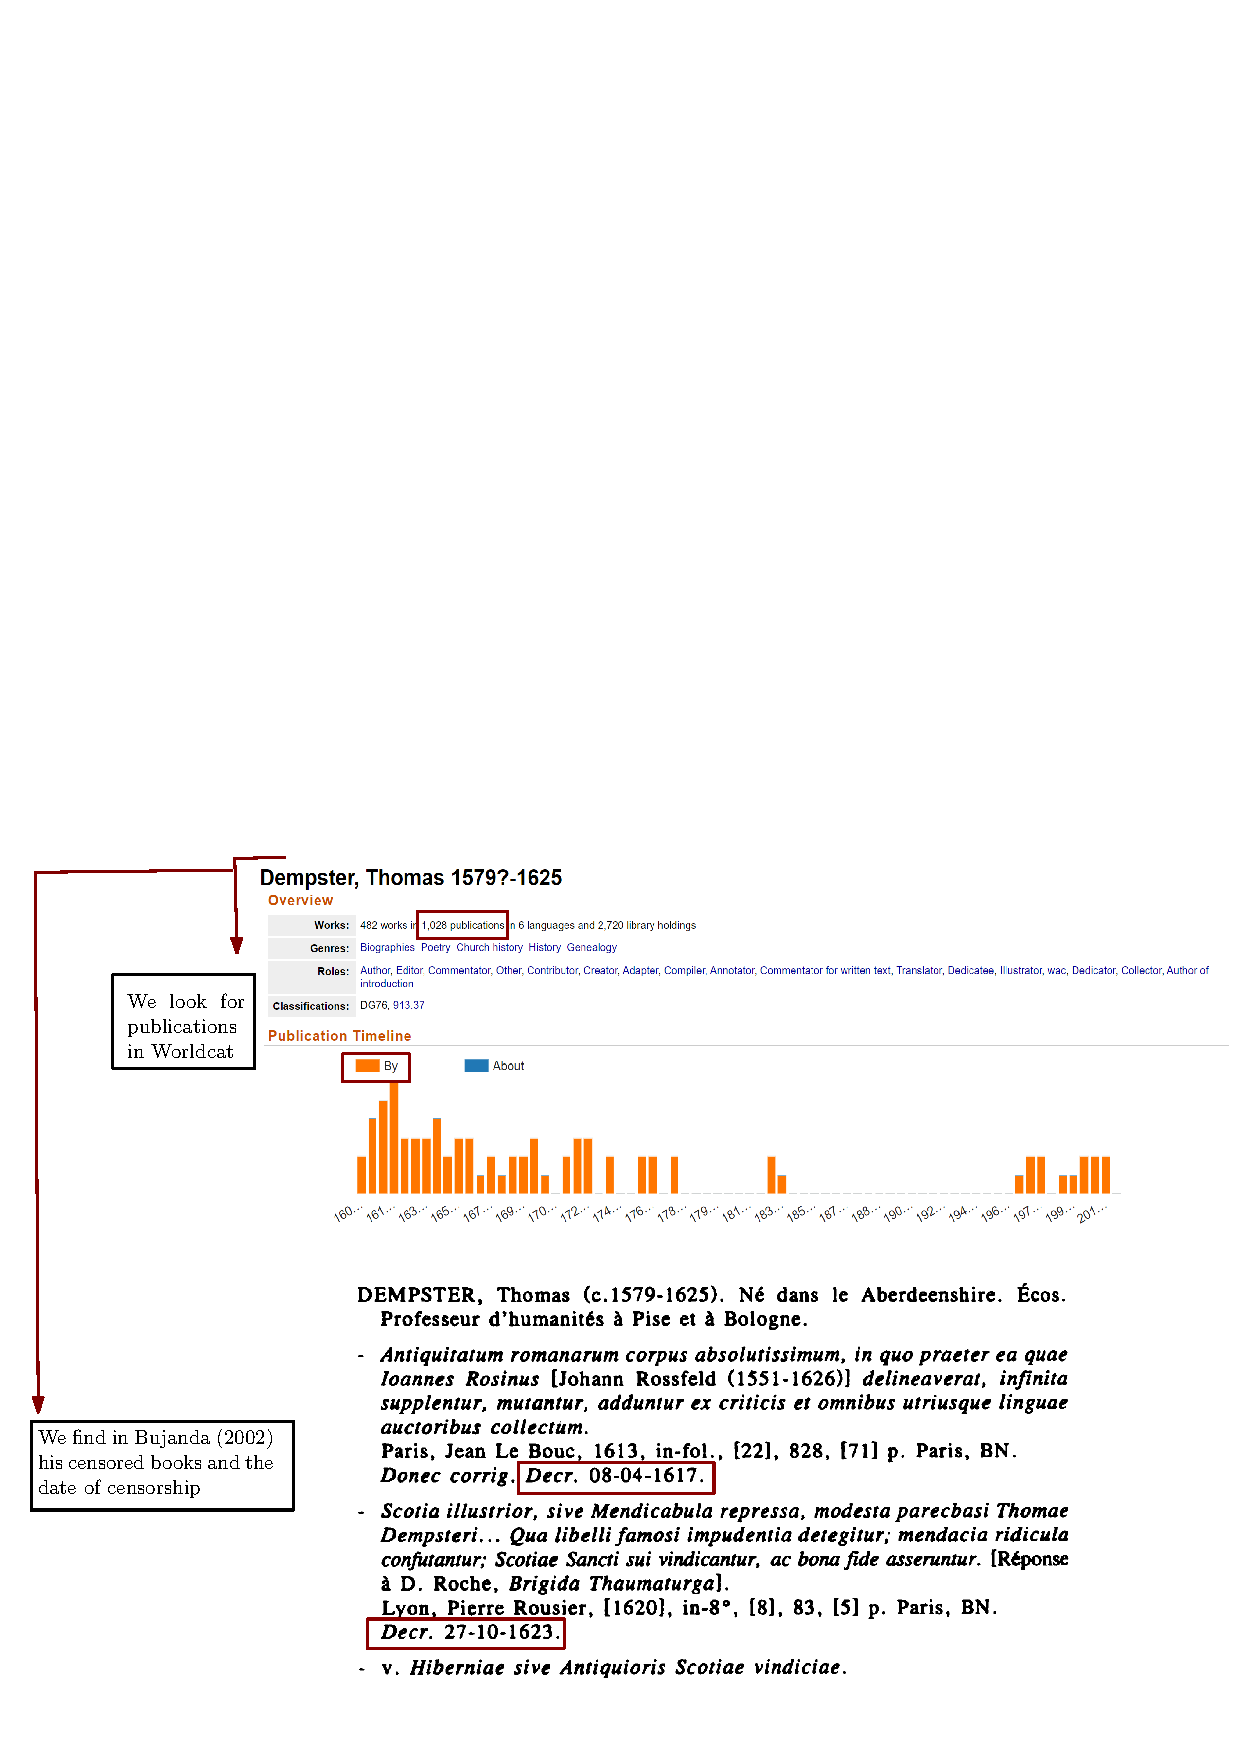
\includegraphics[width=.75\textwidth]{dempster2.pdf}

\end{frame}

	\begin{frame}
\frametitle{Five periods}

 periods: 1:1400-69, 2:1470-1539, 3:1540-1609, 4:1610-79, 5:1680-1749

 Indexes progressively established here and there at the end of period 2, but covering past books as well.

Council of Trent,  established in 1564 the \textit{Index Librorum Prohibitorum}.

The last version of the Index was published in 1948.

 \end{frame}


\begin{frame}
\frametitle{Total number of scholars \& publications by period}

\small
		\begin{tabular}{@{ \extracolsep{1pt}}lcccccccccc}
			\hline
			\hline
			& \multicolumn{5}{c}{Nb. of published scholars}  & \multicolumn{5}{c}{ Median nb. publications per p.}\\
			Period   & 1 &2 & 3 & 4 & 5  & 1 &2 & 3 & 4 & 5\\
			\hline
Ubologna-1088 & 56       & 86       & 79       & 56       & 67       & 34       & 57       & 37       & 16       & 7 \\
Unapoli-1224 & 10       & 20       & 26       & 20       & 18       & 97       & 69       & 17       & 17       & 41 \\
Upadua-1222 & 76       & 131      & 131      & 76       & 79       & 32       & 39       & 41       & 30       & 12 \\
Upavia-1361 & 38       & 71       & 50       & 16       & 8        & 44       & 58       & 36       & 16       & 7 \\
Uroma-1303 & 42       & 61       & 60       & 44       & 40       & 204      & 97       & 67       & 41       & 59 \\
Upisa-1343 & 12       & 38       & 68       & 58       & 36       & 32       & 40       & 20       & 31       & 10 \\
UGregoriana-1556 & 0        & 0        & 64       & 54       & 51       & 0        & 0        & 118      & 55       & 15 \\
StudFlorence-1321 & 42       & 21       & 13       & 14       & 33       & 53       & 116      & 72       & 83       & 12 \\
AcadRicovrati-1599 & 0        & 1        & 71       & 115      & 189      & 0        & 2        & 28       & 36       & 27 \\
AcadCrusca-1583 & 0        & 2        & 38       & 106      & 119      & 0        & 294      & 29       & 30       & 40 \\
\\
Italy    & 206      & 388      & 758      & 751      & 768      & 52       & 60       & 49       & 29       & 20 \\
Europe   & 413      & 1252     & 2835     & 3727     & 5390     & 30       & 50       & 54       & 46       & 44  \\
			\hline
			\hline
	\end{tabular}


\end{frame}



	\begin{frame}
\frametitle{Distribution of published authors by quality. Red: censored. Green: non-censored. }

\parbox{10cm}{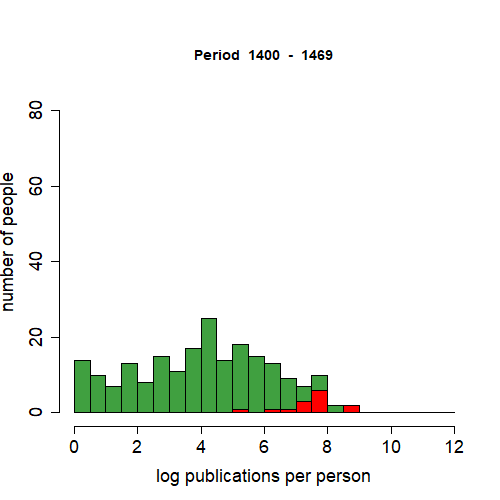
\includegraphics[width=4.95cm,trim=0cm 0cm 0cm 1.5cm, clip]{histo1Q.png}
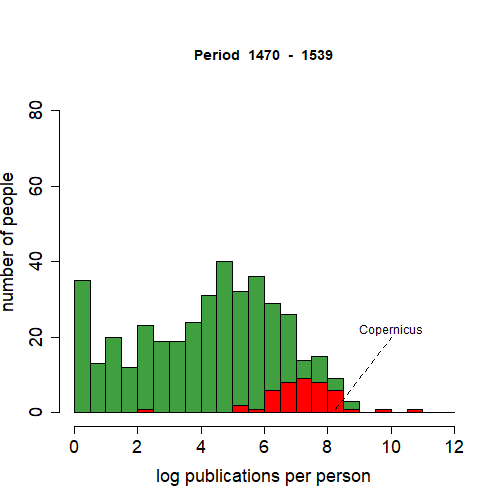
\includegraphics[width=4.95cm,trim=0cm 0cm 0cm 1.5cm, clip]{histo2Q.png}}\;
\parbox{3.6cm}{\begin{flushleft}Censorship concentrated on top scholars for the first periods, then became more uniformly distributed\end{flushleft}}


\end{frame}

	\begin{frame}

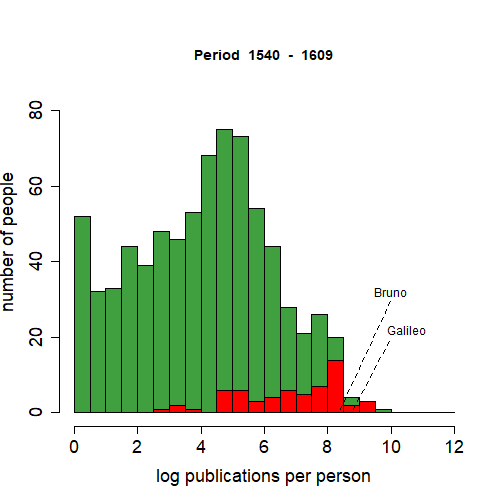
\includegraphics[width=.33\textwidth,trim=0cm 0cm 0cm 1cm, clip]{histo3Q.png}
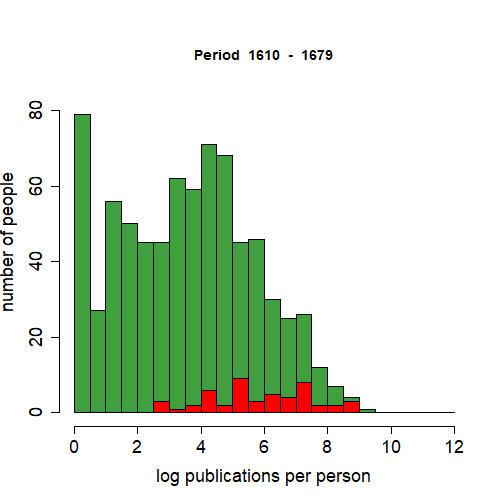
\includegraphics[width=.33\textwidth,trim=0cm 0cm 0cm 1cm, clip]{histo4Q.png}
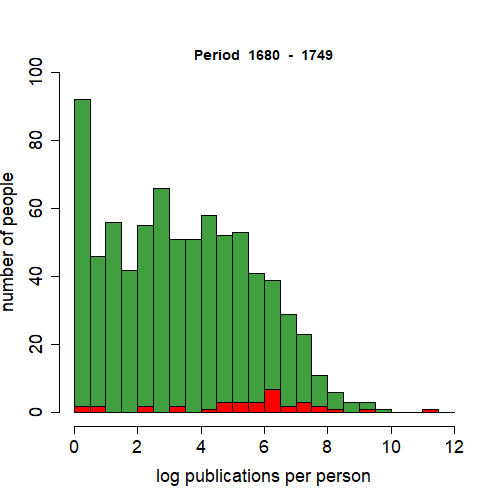
\includegraphics[width=.32\textwidth,trim=0cm 0cm 0cm 1cm, clip]{histo5Q.png}

\end{frame}




	\begin{frame}
\frametitle{Key statistics (moments we will fit)}

%\begin{tabular}{ccccc}
\begin{tabular}{lccccc}
\hline
\hline
Moment description& \multicolumn{5}{c}{Period}\\
   & 1400-69 &1470-1539 & 1540-1609 & 1610-79 & 1680-1749 \\
\hline
Nb published scholars
    &  206     &  388       &  758      &  751     &  768  \\
\% censored scholars
    &  6.8     &  11.08      &  7.92     &  6.66    &  4.56  \\
    \\
Median $p_{it}$ (all)
    &  4.33     &  4.51      &  4.26     &  3.69    &  3.26  \\
Median $p_{it}$ (censored)
    &  7.71     &  7.05      &  7.05     &  5.64    &  5.91  \\
    \\
$75$ percentile $p_{it}$ (all)
    &  5.77     &  5.86      &  5.56     &  5.04    &  5.14  \\
$75$ perc. $p_{it}$ (censored)
    &  7.87     &  7.85      &  8.13     &  7.27    &  6.81  \\
\hline
\hline
\end{tabular}


$p_{it}$: log publications per scholar

\end{frame}

	\begin{frame}
\frametitle{More facts}

After the second period, the percentage of censored authors is shrinking over time.

 Overall quality, measured by median publications per person, is declining over time as well.

Also holds for the top of the distribution, as the 75 percentile also diminishes over the last four periods.

Compatible with the idea of the top innovators' books becoming progressively compliant and of lower quality over time.


\end{frame}


	\begin{frame}
\frametitle{Place of birth of censored (red) and non censored (green) scholars}

\parbox{9cm}{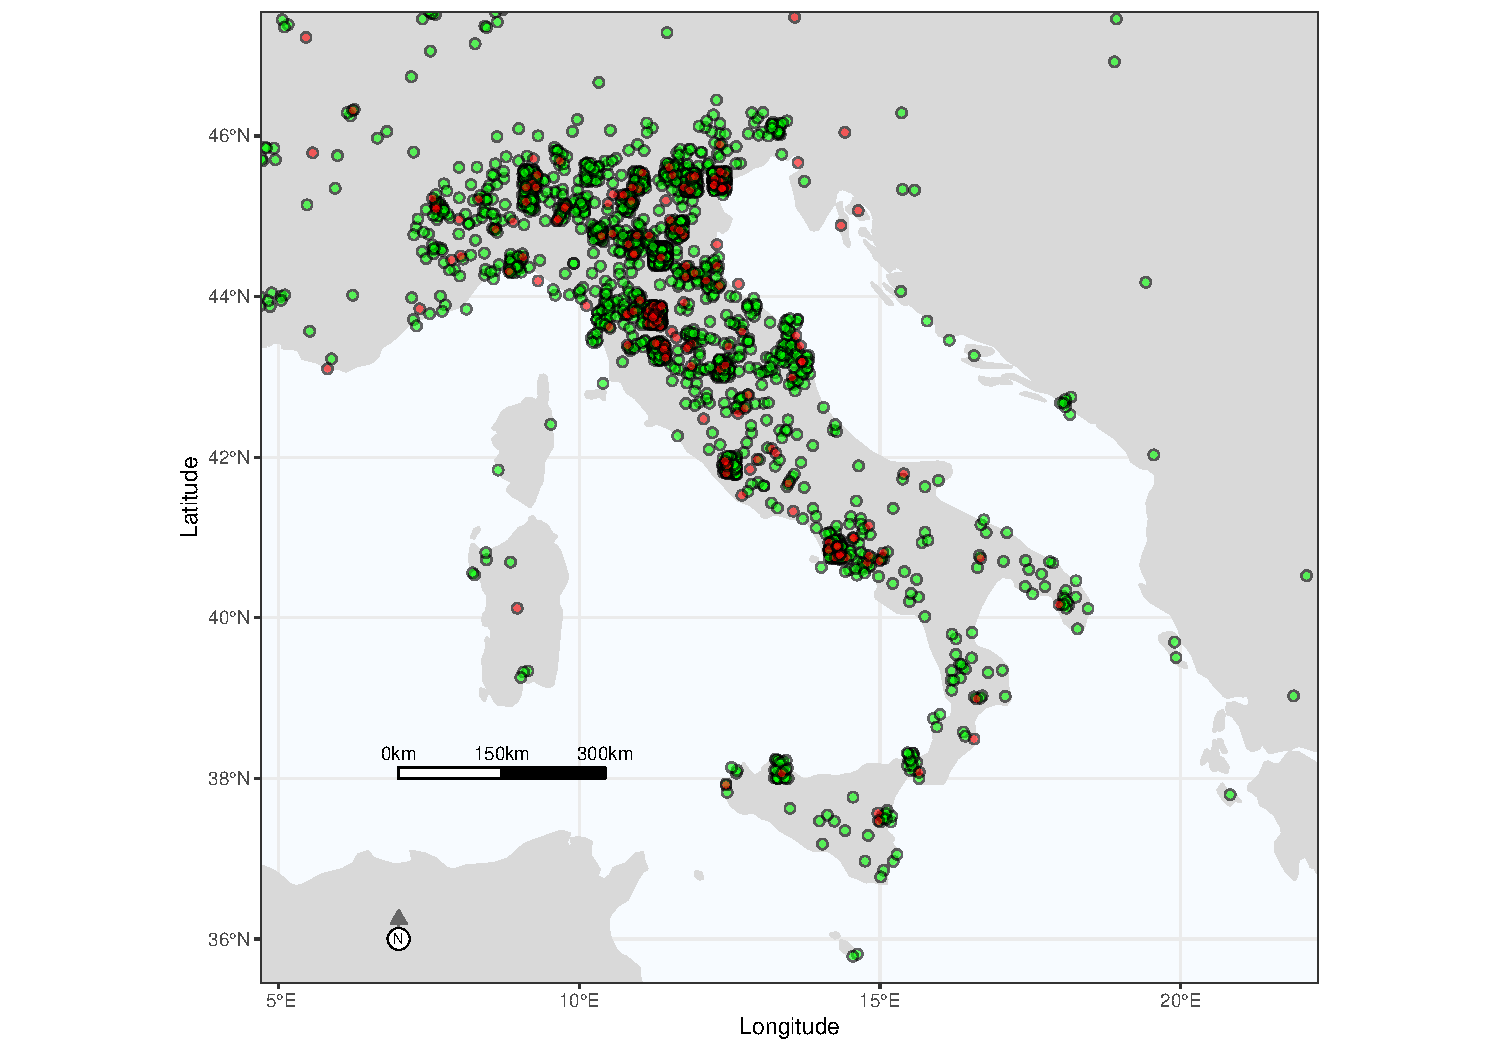
\includegraphics[width=8cm,trim=3cm .6cm 3cm .8cm,clip]{map-italy.pdf}}\;\;
\parbox{4cm}{
Our data cover the whole peninsula and its islands.

\vspace{1cm}Censorship seems to affect all regions rather uniformly.
}
\end{frame}


%%%%%%%%%%%%%%%%%%%%%%%%%%%%%%%%%%%%%%%%%%%%%%%%%%%%%%%%%%%%%%%%%%%%%%%%%%%%%%%%%%%%%%%%%%%%%%%%%%%%%%%%%%%%%%%%%%%%%%%%%%%%%%%%%%%%%%%%%%%%%%%%%%%%%%%
	\section{Model}
	\subsection{}

	\begin{frame}
\frametitle{Persons and Books}

Time is discrete.

 At each date $t$ one generation of $S$ persons is alive.


  Knowledge is embodied in books.

At the beginning of each period,  individuals  learn from $\mu_t$ books.


$\mu_t$: exogenous number of books one can buy during her life.


 Books include more or less relevant content to produce goods and services.


Each book  $i$ has a negative feature $h_i$, say irrelevance.
 The quality of a book is a decreasing function of its irrelevance, with elasticity $\theta$:
\begin{equation}\label{eq:qi}
q_i=h_i^{-\theta}, \;\;\; \theta\in(0,1).
\end{equation}
\end{frame}

	\begin{frame}
\frametitle{Two types of Books}

Books are of two types.


 \textit{Compliant},  superscript ${C}$

  \textit{Revolutionary},  superscript $R$

At the beginning of time $t$, the irrelevance of book $i$ of type $j$ follows an exponential distribution with scale parameter $k_t^j$:
\begin{equation}
h^j_i \sim \exp(k_{t}^j), \quad \text{with} \ j\in \{C,R\}.
\end{equation}
 As
$$
\mbox{E}[h^j_i]=\frac{1}{k^j_{t}},
$$
$k^j_{t}$ measures the average usefulness of knowledge in sector $j$.

\end{frame}

	\begin{frame}
\frametitle{The Fr\'echet Distribution}

The distribution of book quality represents the technology frontier.

Since the irrelevance of books $h_i$ is exponentially distributed and given Equation~(\ref{eq:qi}), the distribution of book quality $q_i$ follows a Fr\'echet distribution with scale parameter ${k^j}^\theta$ and shape parameter $1/\theta$.

Book quality $q^j$ by sector as:
\begin{equation}
E(q^j_i)=\Gamma(1-\theta) \; (k^j)^{\theta} \text{with} \ j\in \{C,R\},
\end{equation}
where $\Gamma(\cdot)$ is the Euler gamma function.
\end{frame}

	\begin{frame}
\frametitle{Best books}

 Share of printers that produced revolutionary books in the previous generation is denoted by  $m_{t}$.

An individual  reads $ \mu_{t+1} m_{t} $ revolutionary books  and $ \mu_{t+1}
 (1-m_{t}) $ compliant books, drawn from their respective distribution.

 Each individual $s$ retains the best book coming from each one of the two distributions:

\begin{align*}	
   \hat{h}^C_s&=\text{min}\{h^C_1,..,h^C_{(1-m_{t}) \mu_{t+1}}\},
 \\ \hat{h}^R_s&=\text{min}\{h^R_1,..,h^R_{ m_{t} \mu_{t+1} }\}.
 \end{align*}

\end{frame}

	\begin{frame}
The exponential distribution satisfies the minimum stability postulate: if $x$ and $y$ are mutually independent random variables, exponentially distributed with parameter $\lambda$, then $\min(x,y)$ is exponentially distributed with parameter $2\lambda$.

\begin{align*}
\min\{h^C_1,..,h^C_{(1-m_{t}) \mu_{t+1}}\}& \sim \exp(k^C_{t} (1-m_{t}) \mu_{t+1}),\;\;\;\mbox{ and }\\
\min\{h^R_1,..,h^R_{ m_{t} \mu_{t+1} }\}& \sim \exp(k^R_{t} m_{t} \mu_{t+1}).
 \end{align*}
Distribution of actual relevance of the best book read by person $s$ follows
\begin{equation}
 \hat{h}^j_s \sim \exp(b_{t+1}^j), \quad \text{with} \ j\in \{C,R\},
\end{equation}
where $b_{t+1}^C$ and $b_{t+1}^R$ are defined as
 \begin{align*}
  b_{t+1}^C&=k_{t}^C (1-m_{t}) \mu_{t+1}, \\
  b_{t+1}^R&=k_{t}^R m_{t}  \mu_{t+1}.
 \end{align*}

\end{frame}


	\begin{frame}
\frametitle{New books}
Later in life, the generation $t+1$ writes new books,  combining their inherited knowledge with a new idea. This new idea is drawn from a distribution whose scale parameter depends on the average quality of the books they have read:
$$
h^j_{sN}\sim  \exp(\nu b^j_{t+1}), \quad \text{with} \ j\in \{C,R\}.
$$
Taking the best of their acquired and new knowledge leads to a book with irrelevance distributed as:
\begin{equation}
\tilde h^j_s=\min(h^j_{sN},\hat h^j_s) \sim  \exp((1+\nu) b^j_{t+1}). \label{eq:writing}
\end{equation}
We can now summarize the dynamics of the two types of knowledge by the dynamics of the scale of their distribution:
 \begin{align}
  k_{t+1}^C&=(1+\nu) k_{t}^C (1-m_{t}) \mu_{t+1},\label{eq:kCtime} \\
  k_{t+1}^R&=(1+\nu) k_{t}^R m_{t} \mu_{t+1}. \label{eq:kRtime}
 \end{align}
\end{frame}



	\begin{frame}
\frametitle{Occupational Choice}

Printers decide whether to be active in the compliant sector or in the revolutionary sector at the beginning of their activity.

Once they have chosen a sector, they would print any author they meet randomly.

They will  determine their sector of activity based on the first author $s$ they meet. This author has written two book projects of quality $q^C_s$ and $q^R_s $. The best will be printed.

Relative price at which revolutionary books are sold is $p$ (exogenous)
\end{frame}


	\begin{frame}
\frametitle{Occupational Choice (2)}

   The probability that the revolutionary book is best is:
\begin{equation}
\text{Prob}\{q^C_i<p q^R_i\}=\text{Prob}\{\tilde{h}^C_s>p^{-1/\theta}\tilde{h}^R_s\}=\frac{b^R_t}{b^R_t+b^C_t p^{-1/\theta}}=m_t.\label{eq:occupation}
\end{equation}


Using the law of large numbers, this probability also defines the share of printers active in the revolutionary sector $m_t$.

$\hat{p}=p^{-1/\theta}$.

The dynamics of knowledge quality (\ref{eq:kCtime}) and (\ref{eq:kRtime}),  together with the occupation choice, imply a static relationship:
\begin{equation}\label{eq:sharer}
m_t=\frac{k^R_t}{k^R_t+\hat{p}k^C_t}
\end{equation}
and initial conditions $k_{1}^C$ and $k_{1}^R$, determine $m_{1}$ .

\end{frame}





	\begin{frame}
\frametitle{The Equilibrium under an Exogenous Church's Behavior}


We start defining $z=k^R/k^C$: From equation (\ref{eq:sharer}) we get
\begin{equation}
m_t=\frac{z_t}{\hat{p}+z_t}\label{eq:sharer2}.
\end{equation}
 We decided to make $m_t$ rather than $z_t$ our main variable for describing the model dynamics because its domain is a bounded set.


We treat $\beta$ as if it was exogenous, and we study the dynamics under this assumption.

Censorship limits the number of revolutionary books that individuals in $t+1$ encounter during their life to $\mu_{t+1} m_t (1-\beta)$ and therefore alters the process of accumulation of revolutionary knowledge, which now follows
\begin{equation}\label{eq:censorship}
k_{t+1}^R=(1+\nu)(1-\beta)k_{t}^R m_{t} \mu_{t+1}, \quad\text{with} \ \beta\in[0,1].
\end{equation}
\end{frame}




	\begin{frame}
\frametitle{The Dynamics under an Exogenous Church's Behavior}

Dividing Equation~(\ref{eq:censorship}) by (\ref{eq:kCtime}) side by side, and substituting the resulting $z_{t+1}$ in (\ref{eq:sharer2}) at time $t+1$, we get the equation that governs the equilibrium dynamics of $m$:
\begin{equation}
m_{t+1}=\frac{(1-\beta) m_t^2}{1-m_t ((\beta -2) m_t+2)}=f(m_t;\beta)\label{eq:lawm}.
\end{equation}


\begin{proposition}
	Given the initial $m_1\in[0,1)$, the long run share of revolutionary authors, $m\equiv\lim_{t\to\infty}m_t$, is given by
	\begin{itemize}
    \item[i)]$m=0$ if $m_1<1/(2-\beta)$ (Compliant steady state),
    \item[ii)] $m=1$ if $m_1>1/(2-\beta)$ (Revolutionary steady state),
     \item[iii)]$m=m_1$ if $m_1=1/(2-\beta)$ (Unstable steady state).
	\end{itemize}
	 \label{proposition:dynex}
\end{proposition}


%Notice finally that the path of $m_t$ does not depend on the process $\mu_t$, but quality levels $k^R_t$ and $k^C_t$ do.
\end{frame}



	\begin{frame}

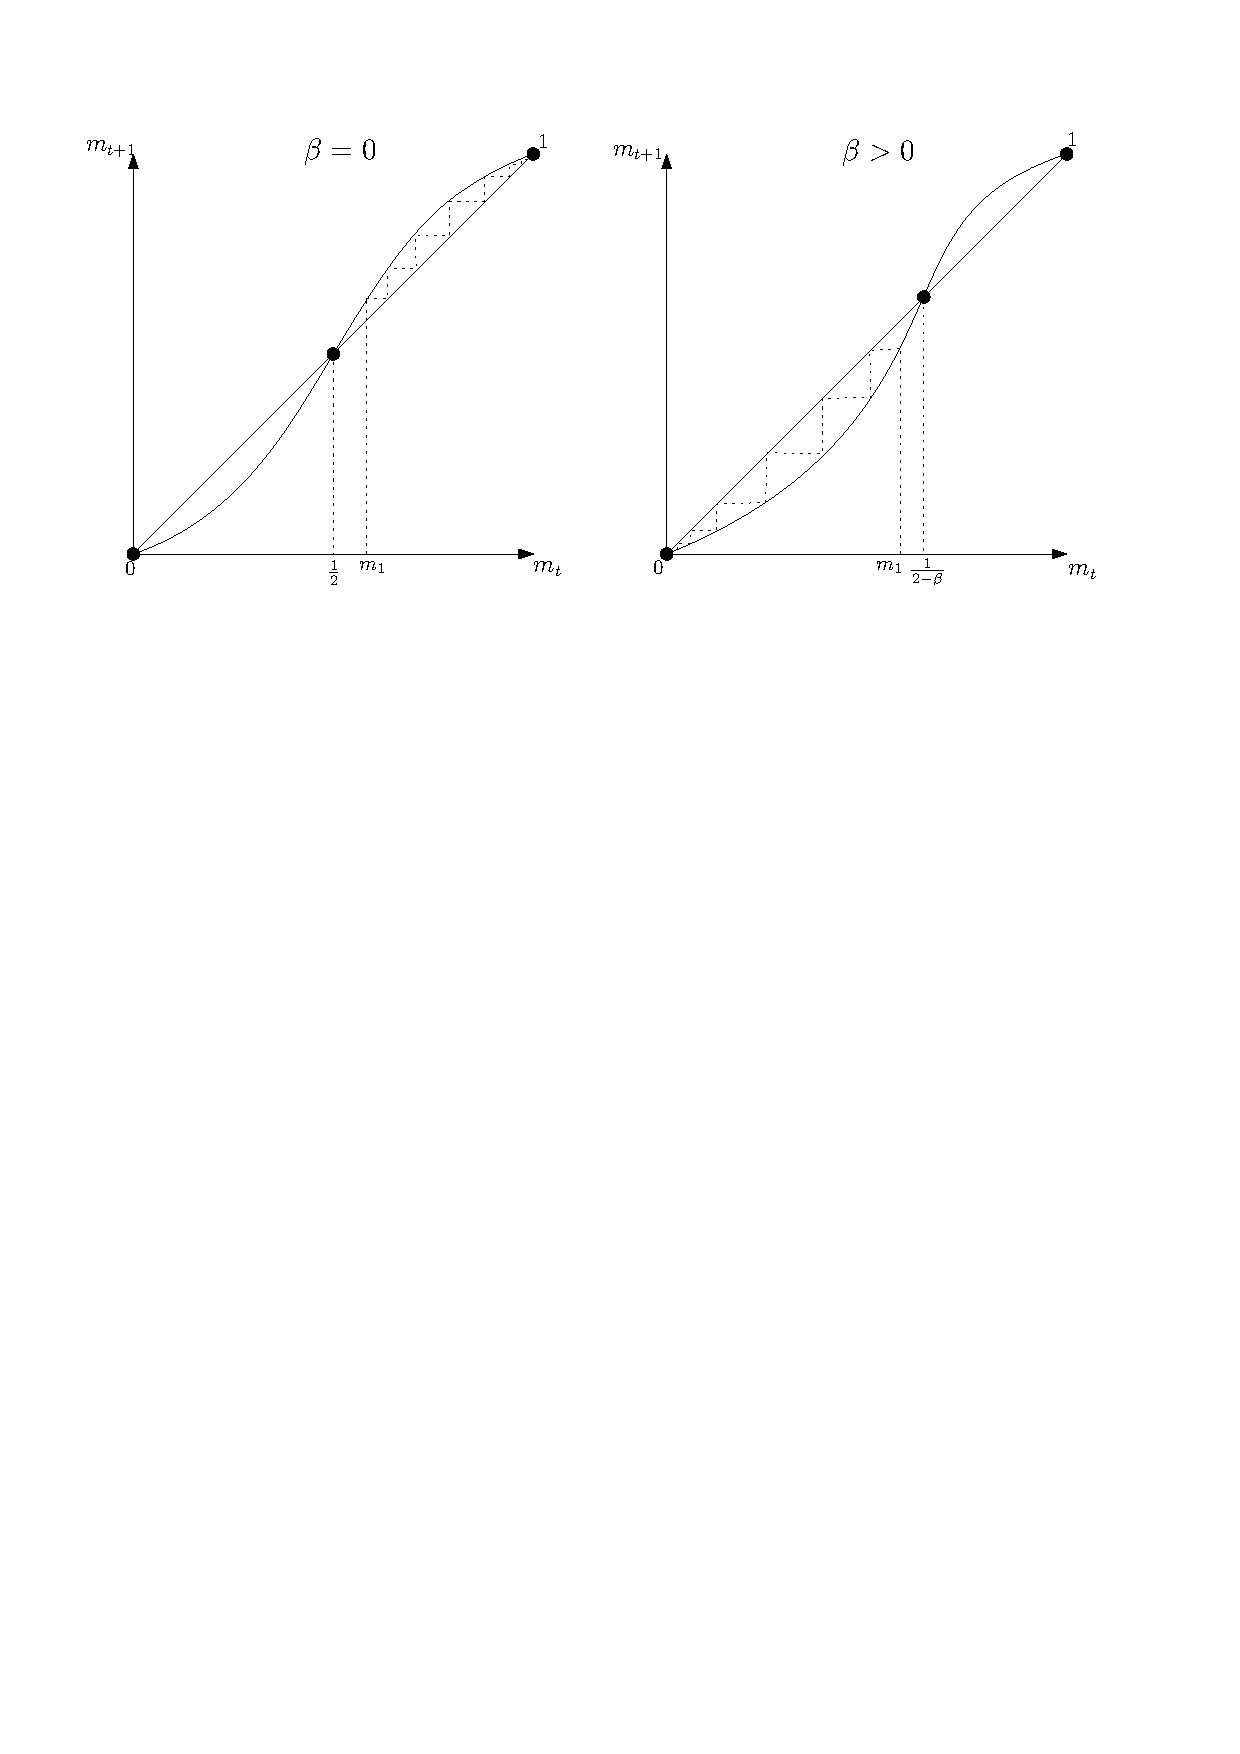
\includegraphics[width=13cm]{dynamics-m.pdf}
\end{frame}


	\begin{frame}
\frametitle{The Equilibrium under  Optimizing Church's Behavior}

Endogenize the timing of censorship: Church cannot enforce any censorship before having paid a fixed cost $\psi$.

  After having paid $\psi$, she can impose a rate of censorship up to $\overline{\beta}$.

   The Church cares about the share of compliant books in the economy:  $u(1-m_t)$.
\begin{align*}	
	V(m_{t})&=\max[V^N(m_{t}),V^C(m_{t})-\psi],\\
V^{N}(m_{t})&=u(1-m_{t})+\delta V(m_{t+1})	\;\;\;
	 \text{s.t.}\quad m_{t+1}=f(m_{t};0),\\
V^{C}(m_{t})&=\max_{0\leq\beta_t\leq\overline{\beta}}u(1-m_{t})+\delta V^C(m_{t+1})\;\;\;	
	 \text{s.t.}\quad m_{t+1}=f(m_{t};\beta_t).
\end{align*}
the Church has to choose between paying a fixed cost today for enjoying a lower share of revolutionary books in the future and postponing such payment.

\end{frame}




	\begin{frame}
\frametitle{The Dynamics  under  Optimizing Church's Behavior}

The Church's decision to start censoring also depends on the initial level of revolutionary books $m_{1}$.

\begin{proposition}7
\label{proposition:tooLate}
If $\psi>0$, then there exist $\tilde{m}>0$ and $1>\breve{m}>0$ such that
\begin{itemize}
\item[i)] If $m_1<\min(1/2,\tilde{m})$ then $\beta_t=0$ for each $t\geq1$ (No need to censor),
\item[ii)] If $m_1>\max(1/2,\breve{m})$ then $\beta_t=0$ for each $t\geq1$ (Too late to censor).
\end{itemize}
\end{proposition}


\begin{proposition}
\label{proposition:window}
There exists $\overline{\psi}$ such that for each $\psi<\overline{\psi},\;\text{there also exists} \;\overline{m},\hat{m}$ such that for $\hat{m}>m_{1}>\overline{m}$, $\beta_1=\overline{\beta}$ holds (window of censorship).
\end{proposition}


\end{frame}


%%%%%%%%%%%%%%%%%%%%%%%%%%%%%%%%%%%%%%%%%%%%%%%%%%%%%%%%%%%%%%%%%%%%%%%%%%%%%%%%%%%%%%%%%%%%%%%%%%%%%%%%%%%%%%%%%%%%%%%%%%%%%%%%%%%%%%%%%%%%%%%%%%%%%%%
	\section{Estimation}
	\subsection{}

	\begin{frame}
\frametitle{Mapping Model to Data}

Specify the relationship between model periods and their empirical counterpart:

\begin{tabular}{ccccc}
\hline\hline
$t$         &   years       & rate of censorship $\beta $  & share of censored authors & $\mu_t$ \\
\hline
1           & 1400-1469     & 0                            & 0                        & 1.000\\
2           & 1470-1539     & 0                            & $m_2\overline{\beta}$    &  0.878\\
3           & 1540-1609     & $\overline{\beta}$           & $m_3\overline{\beta}$    & 0.787\\
4           & 1610-1679     & $\overline{\beta}$           & $m_4\overline{\beta}$    & 0.828\\
5           & 1680-1749     & $\overline{\beta}$           & $m_5\overline{\beta}$    & 0.851\\
\hline\hline\end{tabular}

note: censorship in period 3 affects books written in period 2.
\end{frame}


	\begin{frame}
\frametitle{Estimation strategy}

Set one parameter following the literature ($\delta$).

Estimate six parameters using a minimum distance estimation procedure, under the assumption that censorship kicks in mid $16^{th}$ century as in the data.
$$\vartheta=[k^C_1,k^R_1,\theta,\overline{\beta},\nu,p]$$

 Set  parameter $\psi$ to match the timing of the introduction of censorship.

\end{frame}

	\begin{frame}
\frametitle{Minimum Distance Estimation}

 Minimizing the distance between 14 empirical and theoretical moments, implying thus 8 (=14-6) over\-identifying restrictions.

 \begin{equation}
\Omega(\vartheta)= (\mathbf{m}-\mathbf{m}_\vartheta)'\mathbf{W}(\mathbf{m}-\mathbf{m}_\vartheta),
\end{equation}

Moments $\mathbf{m}$ to match:

Five moments are the median of the quality of all authors, and five other moments are their  $75^{th}$ percentile. The last four moments are the share of censored authors $m_t \overline{\beta}$ for $t=2,3,4,5$.

Distribution of the quality of all authors, $q_{it}$, obtained by drawing with probability $m_t$ from the distribution of $q^R_t$ (i.e. a Fr\'echet($(k_t^R)^\theta,1/\theta$)) and with probability $(1-m_t)$  from the distribution of $q^C_t$.

\end{frame}

	\begin{frame}
\frametitle{Estimation Results}

      \begin{tabular}{@{\extracolsep{5pt}}l c c c c}
      \hline\hline%inserts double horizontal lines
      \rule{-4pt}{2.5ex}
       Calibrated Parameters &  & Value & Std. Errors & Target \\ [0.05ex] % inserts table
       \hline
      \rule{-4pt}{2.5ex}
       Discount Factor  & $\delta$   &0.06& -  &RBC lit.\\[0.15ex]
       Fixed Cost of Censorship  & $\hat{\psi}$   &(\hspace{-0.1cm} 1.031 - 1.034 \hspace{-0.1cm})& - &Index set-up \\[0.15ex]
       \hline % inserts single horizontal line
       \rule{-4pt}{2.5ex}
       Estimated Parameters &  & Value & Std. Errors & Target  \\ [0.05ex] % inserts table
        %heading
      \hline % inserts single horizontal line
      \rule{-4pt}{2.5ex}
      Compliant knowledge in 1  & $k^C_1$   & 16.6 & 1.21  &  $\Omega(\vartheta)$  \\[0.15ex]
      Rev. knowledge in 1  & $k^R_1$   & 117.5 & 10.86  & $\Omega(\vartheta)$ \\[0.15ex]
      Productivity of books  & $\theta$   & 0.34 &  0.017  & $\Omega(\vartheta)$\\[0.15ex]
      Max Censorship  & $\overline{\beta}$   & 0.19 &  0.015 & $\Omega(\vartheta)$\\[0.15ex]
      Knowledge Growth   & $\nu$   & 1.45 &  0.071  & $\Omega(\vartheta)$\\[0.15ex]
      Price of rev. books   & $p$   & 0.52 &  0.019  & $\Omega(\vartheta)$\\[0.15ex]
      \hline\hline
      \end{tabular}



 \end{frame}

	\begin{frame}
\frametitle{Model fit - Data (solid) and simulations (dashed)}

\parbox{.49\textwidth}{
		\centering
		{Overall scholars\\quality: \textcolor{red}{median}, \textcolor{blue}{$75^{th}$ percentile}}

\scalebox{0.45}{% Created by tikzDevice version 0.12.3.1 on 2022-09-19 21:45:14
% !TEX encoding = UTF-8 Unicode
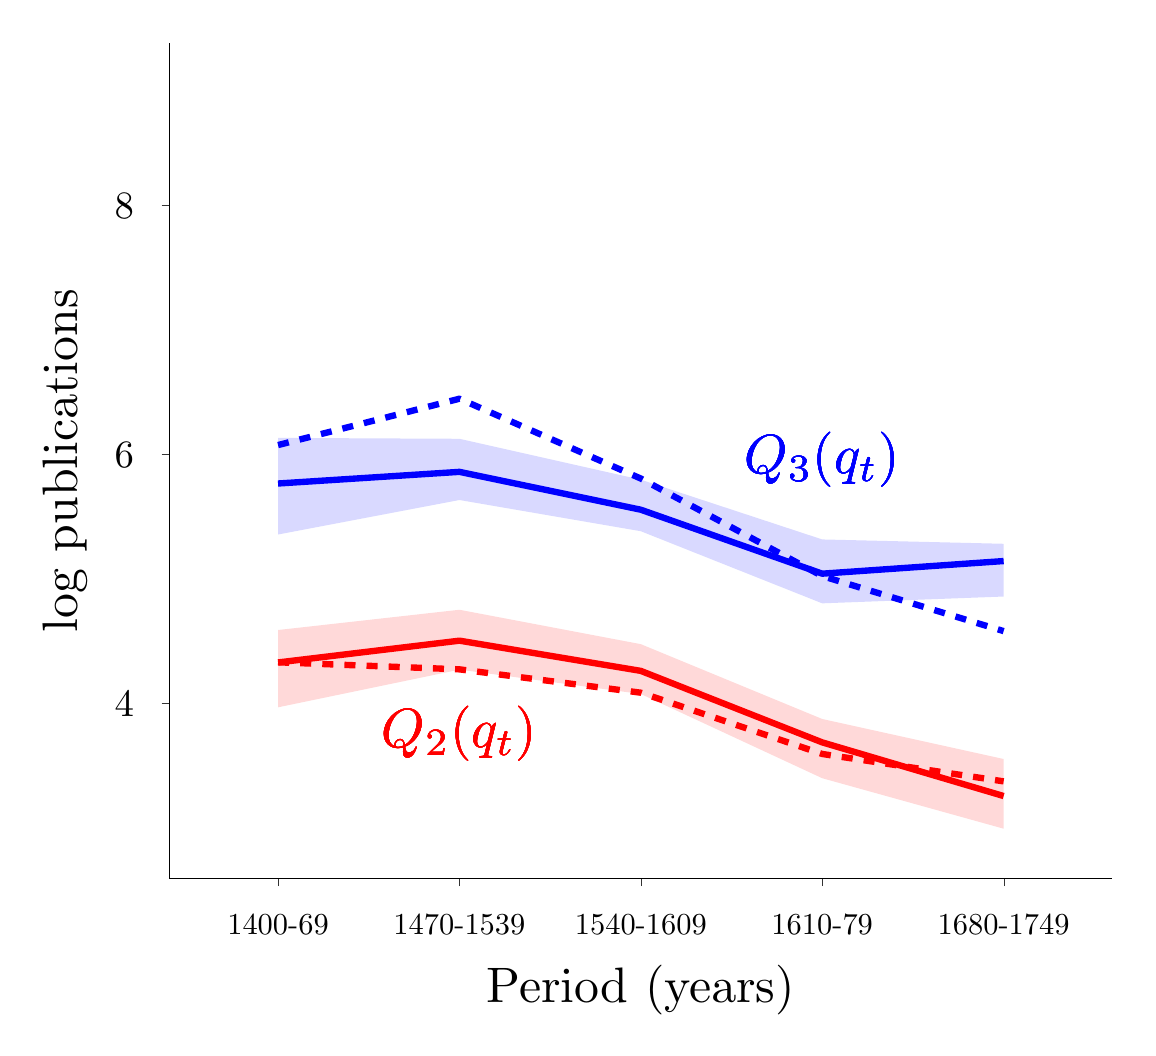
\begin{tikzpicture}[x=1pt,y=1pt]
\definecolor{fillColor}{RGB}{255,255,255}
\path[use as bounding box,fill=fillColor,fill opacity=0.00] (0,0) rectangle (397.48,361.35);
\begin{scope}
\path[clip] (  0.00,  0.00) rectangle (397.48,361.35);
\definecolor{drawColor}{RGB}{255,255,255}
\definecolor{fillColor}{RGB}{255,255,255}

\path[draw=drawColor,line width= 0.1pt,line join=round,line cap=round,fill=fillColor] (  0.00,  0.00) rectangle (397.48,361.35);
\end{scope}
\begin{scope}
\path[clip] ( 51.14, 53.86) rectangle (391.98,355.85);
\definecolor{fillColor}{RGB}{255,255,255}

\path[fill=fillColor] ( 51.14, 53.86) rectangle (391.98,355.85);
\definecolor{fillColor}{RGB}{255,0,0}

\path[fill=fillColor,fill opacity=0.15] ( 90.47,143.69) --
	(156.02,151.01) --
	(221.56,138.58) --
	(287.11,111.54) --
	(352.66, 97.08) --
	(352.66, 71.90) --
	(287.11, 90.14) --
	(221.56,120.58) --
	(156.02,129.37) --
	( 90.47,115.76) --
	cycle;

\path[] ( 90.47,143.69) --
	(156.02,151.01) --
	(221.56,138.58) --
	(287.11,111.54) --
	(352.66, 97.08);

\path[] (352.66, 71.90) --
	(287.11, 90.14) --
	(221.56,120.58) --
	(156.02,129.37) --
	( 90.47,115.76);
\definecolor{drawColor}{RGB}{255,0,0}

\path[draw=drawColor,line width= 2.3pt,line join=round] ( 90.47,131.97) --
	(156.02,139.84) --
	(221.56,128.92) --
	(287.11,103.09) --
	(352.66, 83.70);

\path[draw=drawColor,line width= 2.3pt,dash pattern=on 4pt off 4pt ,line join=round] ( 90.47,132.03) --
	(156.02,129.48) --
	(221.56,121.04) --
	(287.11, 98.90) --
	(352.66, 89.00);
\definecolor{fillColor}{RGB}{0,0,255}

\path[fill=fillColor,fill opacity=0.15] ( 90.47,213.11) --
	(156.02,212.79) --
	(221.56,198.01) --
	(287.11,176.42) --
	(352.66,174.85) --
	(352.66,155.79) --
	(287.11,153.33) --
	(221.56,179.39) --
	(156.02,190.67) --
	( 90.47,178.20) --
	cycle;

\path[] ( 90.47,213.11) --
	(156.02,212.79) --
	(221.56,198.01) --
	(287.11,176.42) --
	(352.66,174.85);

\path[] (352.66,155.79) --
	(287.11,153.33) --
	(221.56,179.39) --
	(156.02,190.67) --
	( 90.47,178.20);
\definecolor{drawColor}{RGB}{0,0,255}

\path[draw=drawColor,line width= 2.3pt,line join=round] ( 90.47,196.63) --
	(156.02,200.84) --
	(221.56,187.16) --
	(287.11,164.05) --
	(352.66,168.61);

\path[draw=drawColor,line width= 2.3pt,dash pattern=on 4pt off 4pt ,line join=round] ( 90.47,210.52) --
	(156.02,227.27) --
	(221.56,198.42) --
	(287.11,163.18) --
	(352.66,143.30);

\node[text=drawColor,anchor=base,inner sep=0pt, outer sep=0pt, scale=  1.99] at (287.11,200.25) {$Q_3(q_t)$};

\node[text=drawColor,anchor=base,inner sep=0pt, outer sep=0pt, scale=  1.99] at (287.11,200.25) {$Q_3(q_t)$};

\node[text=drawColor,anchor=base,inner sep=0pt, outer sep=0pt, scale=  1.99] at (287.11,200.25) {$Q_3(q_t)$};

\node[text=drawColor,anchor=base,inner sep=0pt, outer sep=0pt, scale=  1.99] at (287.11,200.25) {$Q_3(q_t)$};

\node[text=drawColor,anchor=base,inner sep=0pt, outer sep=0pt, scale=  1.99] at (287.11,200.25) {$Q_3(q_t)$};
\definecolor{drawColor}{RGB}{255,0,0}

\node[text=drawColor,anchor=base,inner sep=0pt, outer sep=0pt, scale=  1.99] at (156.02,101.23) {$Q_2(q_t)$};

\node[text=drawColor,anchor=base,inner sep=0pt, outer sep=0pt, scale=  1.99] at (156.02,101.23) {$Q_2(q_t)$};

\node[text=drawColor,anchor=base,inner sep=0pt, outer sep=0pt, scale=  1.99] at (156.02,101.23) {$Q_2(q_t)$};

\node[text=drawColor,anchor=base,inner sep=0pt, outer sep=0pt, scale=  1.99] at (156.02,101.23) {$Q_2(q_t)$};

\node[text=drawColor,anchor=base,inner sep=0pt, outer sep=0pt, scale=  1.99] at (156.02,101.23) {$Q_2(q_t)$};
\end{scope}
\begin{scope}
\path[clip] (  0.00,  0.00) rectangle (397.48,361.35);
\definecolor{drawColor}{RGB}{0,0,0}

\path[draw=drawColor,line width= 0.1pt,line join=round] ( 51.14, 53.86) --
	( 51.14,355.85);
\end{scope}
\begin{scope}
\path[clip] (  0.00,  0.00) rectangle (397.48,361.35);
\definecolor{drawColor}{RGB}{0,0,0}

\node[text=drawColor,anchor=base east,inner sep=0pt, outer sep=0pt, scale=  1.40] at ( 38.39,112.27) {4};

\node[text=drawColor,anchor=base east,inner sep=0pt, outer sep=0pt, scale=  1.40] at ( 38.39,202.28) {6};

\node[text=drawColor,anchor=base east,inner sep=0pt, outer sep=0pt, scale=  1.40] at ( 38.39,292.30) {8};
\end{scope}
\begin{scope}
\path[clip] (  0.00,  0.00) rectangle (397.48,361.35);
\definecolor{drawColor}{gray}{0.20}

\path[draw=drawColor,line width= 0.1pt,line join=round] ( 48.39,117.09) --
	( 51.14,117.09);

\path[draw=drawColor,line width= 0.1pt,line join=round] ( 48.39,207.11) --
	( 51.14,207.11);

\path[draw=drawColor,line width= 0.1pt,line join=round] ( 48.39,297.12) --
	( 51.14,297.12);
\end{scope}
\begin{scope}
\path[clip] (  0.00,  0.00) rectangle (397.48,361.35);
\definecolor{drawColor}{RGB}{0,0,0}

\path[draw=drawColor,line width= 0.1pt,line join=round] ( 51.14, 53.86) --
	(391.98, 53.86);
\end{scope}
\begin{scope}
\path[clip] (  0.00,  0.00) rectangle (397.48,361.35);
\definecolor{drawColor}{gray}{0.20}

\path[draw=drawColor,line width= 0.1pt,line join=round] ( 90.47, 51.11) --
	( 90.47, 53.86);

\path[draw=drawColor,line width= 0.1pt,line join=round] (156.02, 51.11) --
	(156.02, 53.86);

\path[draw=drawColor,line width= 0.1pt,line join=round] (221.56, 51.11) --
	(221.56, 53.86);

\path[draw=drawColor,line width= 0.1pt,line join=round] (287.11, 51.11) --
	(287.11, 53.86);

\path[draw=drawColor,line width= 0.1pt,line join=round] (352.66, 51.11) --
	(352.66, 53.86);
\end{scope}
\begin{scope}
\path[clip] (  0.00,  0.00) rectangle (397.48,361.35);
\definecolor{drawColor}{RGB}{0,0,0}

\node[text=drawColor,anchor=base,inner sep=0pt, outer sep=0pt, scale=  1.10] at ( 90.47, 33.53) {1400-69};

\node[text=drawColor,anchor=base,inner sep=0pt, outer sep=0pt, scale=  1.10] at (156.02, 33.53) {1470-1539};

\node[text=drawColor,anchor=base,inner sep=0pt, outer sep=0pt, scale=  1.10] at (221.56, 33.53) {1540-1609};

\node[text=drawColor,anchor=base,inner sep=0pt, outer sep=0pt, scale=  1.10] at (287.11, 33.53) {1610-79};

\node[text=drawColor,anchor=base,inner sep=0pt, outer sep=0pt, scale=  1.10] at (352.66, 33.53) {1680-1749};
\end{scope}
\begin{scope}
\path[clip] (  0.00,  0.00) rectangle (397.48,361.35);
\definecolor{drawColor}{RGB}{0,0,0}

\node[text=drawColor,anchor=base,inner sep=0pt, outer sep=0pt, scale=  1.80] at (221.56,  9.00) {Period (years)};
\end{scope}
\begin{scope}
\path[clip] (  0.00,  0.00) rectangle (397.48,361.35);
\definecolor{drawColor}{RGB}{0,0,0}

\node[text=drawColor,rotate= 90.00,anchor=base,inner sep=0pt, outer sep=0pt, scale=  1.80] at ( 17.90,204.86) {log publications};
\end{scope}
\end{tikzpicture}
}
}
\parbox{.49\textwidth}{
		\centering
{\% censored scholars\\
\textcolor{white}{a}}

\scalebox{0.45}{% Created by tikzDevice version 0.12.3.1 on 2022-09-19 22:27:54
% !TEX encoding = UTF-8 Unicode
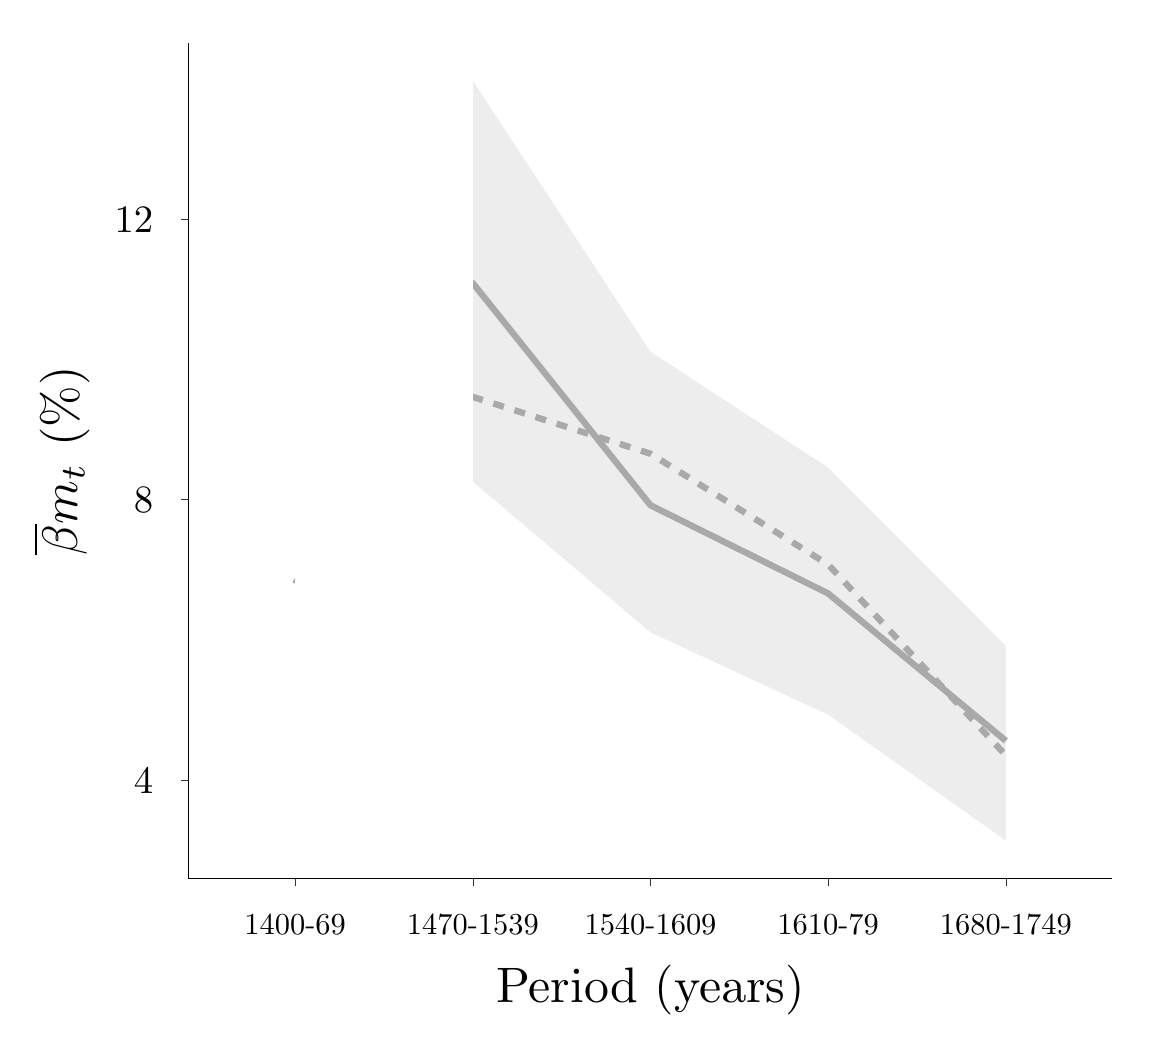
\begin{tikzpicture}[x=1pt,y=1pt]
\definecolor{fillColor}{RGB}{255,255,255}
\path[use as bounding box,fill=fillColor,fill opacity=0.00] (0,0) rectangle (397.48,361.35);
\begin{scope}
\path[clip] (  0.00,  0.00) rectangle (397.48,361.35);
\definecolor{drawColor}{RGB}{255,255,255}
\definecolor{fillColor}{RGB}{255,255,255}

\path[draw=drawColor,line width= 0.1pt,line join=round,line cap=round,fill=fillColor] (  0.00,  0.00) rectangle (397.48,361.35);
\end{scope}
\begin{scope}
\path[clip] ( 58.14, 53.86) rectangle (391.98,355.85);
\definecolor{fillColor}{RGB}{255,255,255}

\path[fill=fillColor] ( 58.14, 53.86) rectangle (391.98,355.85);
\definecolor{fillColor}{RGB}{169,169,169}

\path[fill=fillColor,fill opacity=0.20] ( 96.66,263.42) --
	(160.86,342.12) --
	(225.06,244.23) --
	(289.26,202.36) --
	(353.46,137.94) --
	(353.46, 67.59) --
	(289.26,113.10) --
	(225.06,142.83) --
	(160.86,197.32) --
	( 96.66, 75.91) --
	cycle;

\path[] ( 96.66,263.42) --
	(160.86,342.12) --
	(225.06,244.23) --
	(289.26,202.36) --
	(353.46,137.94);

\path[] (353.46, 67.59) --
	(289.26,113.10) --
	(225.06,142.83) --
	(160.86,197.32) --
	( 96.66, 75.91);
\definecolor{drawColor}{RGB}{169,169,169}

\path[draw=drawColor,line width= 2.3pt,line join=round] ( 96.66,160.39) --
	(160.86,269.05) --
	(225.06,188.77) --
	(289.26,156.89) --
	(353.46,103.64);

\path[draw=drawColor,line width= 2.3pt,dash pattern=on 4pt off 4pt ,line join=round] ( 96.66,226.06) --
	(160.86,227.93) --
	(225.06,207.39) --
	(289.26,167.35) --
	(353.46, 98.39);
\definecolor{fillColor}{RGB}{255,255,255}

\path[fill=fillColor] ( 96.66, 53.86) rectangle (160.86,355.85);

\path[fill=fillColor] ( 96.66, 53.86) rectangle (160.86,355.85);

\path[fill=fillColor] ( 96.66, 53.86) rectangle (160.86,355.85);

\path[fill=fillColor] ( 96.66, 53.86) rectangle (160.86,355.85);

\path[fill=fillColor] ( 96.66, 53.86) rectangle (160.86,355.85);
\end{scope}
\begin{scope}
\path[clip] (  0.00,  0.00) rectangle (397.48,361.35);
\definecolor{drawColor}{RGB}{0,0,0}

\path[draw=drawColor,line width= 0.1pt,line join=round] ( 58.14, 53.86) --
	( 58.14,355.85);
\end{scope}
\begin{scope}
\path[clip] (  0.00,  0.00) rectangle (397.48,361.35);
\definecolor{drawColor}{RGB}{0,0,0}

\node[text=drawColor,anchor=base east,inner sep=0pt, outer sep=0pt, scale=  1.40] at ( 45.39, 84.70) {4};

\node[text=drawColor,anchor=base east,inner sep=0pt, outer sep=0pt, scale=  1.40] at ( 45.39,186.09) {8};

\node[text=drawColor,anchor=base east,inner sep=0pt, outer sep=0pt, scale=  1.40] at ( 45.39,287.49) {12};
\end{scope}
\begin{scope}
\path[clip] (  0.00,  0.00) rectangle (397.48,361.35);
\definecolor{drawColor}{gray}{0.20}

\path[draw=drawColor,line width= 0.1pt,line join=round] ( 55.39, 89.52) --
	( 58.14, 89.52);

\path[draw=drawColor,line width= 0.1pt,line join=round] ( 55.39,190.91) --
	( 58.14,190.91);

\path[draw=drawColor,line width= 0.1pt,line join=round] ( 55.39,292.31) --
	( 58.14,292.31);
\end{scope}
\begin{scope}
\path[clip] (  0.00,  0.00) rectangle (397.48,361.35);
\definecolor{drawColor}{RGB}{0,0,0}

\path[draw=drawColor,line width= 0.1pt,line join=round] ( 58.14, 53.86) --
	(391.98, 53.86);
\end{scope}
\begin{scope}
\path[clip] (  0.00,  0.00) rectangle (397.48,361.35);
\definecolor{drawColor}{gray}{0.20}

\path[draw=drawColor,line width= 0.1pt,line join=round] ( 96.66, 51.11) --
	( 96.66, 53.86);

\path[draw=drawColor,line width= 0.1pt,line join=round] (160.86, 51.11) --
	(160.86, 53.86);

\path[draw=drawColor,line width= 0.1pt,line join=round] (225.06, 51.11) --
	(225.06, 53.86);

\path[draw=drawColor,line width= 0.1pt,line join=round] (289.26, 51.11) --
	(289.26, 53.86);

\path[draw=drawColor,line width= 0.1pt,line join=round] (353.46, 51.11) --
	(353.46, 53.86);
\end{scope}
\begin{scope}
\path[clip] (  0.00,  0.00) rectangle (397.48,361.35);
\definecolor{drawColor}{RGB}{0,0,0}

\node[text=drawColor,anchor=base,inner sep=0pt, outer sep=0pt, scale=  1.10] at ( 96.66, 33.53) {1400-69};

\node[text=drawColor,anchor=base,inner sep=0pt, outer sep=0pt, scale=  1.10] at (160.86, 33.53) {1470-1539};

\node[text=drawColor,anchor=base,inner sep=0pt, outer sep=0pt, scale=  1.10] at (225.06, 33.53) {1540-1609};

\node[text=drawColor,anchor=base,inner sep=0pt, outer sep=0pt, scale=  1.10] at (289.26, 33.53) {1610-79};

\node[text=drawColor,anchor=base,inner sep=0pt, outer sep=0pt, scale=  1.10] at (353.46, 33.53) {1680-1749};
\end{scope}
\begin{scope}
\path[clip] (  0.00,  0.00) rectangle (397.48,361.35);
\definecolor{drawColor}{RGB}{0,0,0}

\node[text=drawColor,anchor=base,inner sep=0pt, outer sep=0pt, scale=  1.80] at (225.06,  9.00) {Period (years)};
\end{scope}
\begin{scope}
\path[clip] (  0.00,  0.00) rectangle (397.48,361.35);
\definecolor{drawColor}{RGB}{0,0,0}

\node[text=drawColor,rotate= 90.00,anchor=base,inner sep=0pt, outer sep=0pt, scale=  1.80] at ( 17.90,204.86) {$\overline{\beta}m_t$ (\%)};
\end{scope}
\end{tikzpicture}
}
}


 \end{frame}

	\begin{frame}
\frametitle{over-identification checks - Data (solid) and simulations (dashed)}

\parbox{.49\textwidth}{
		\centering
{Censored scholars\\quality: \textcolor{red}{median}, \textcolor{blue}{$75^{th}$ percentile}}

\scalebox{0.45}{% Created by tikzDevice version 0.12.3.1 on 2022-09-19 22:27:53
% !TEX encoding = UTF-8 Unicode
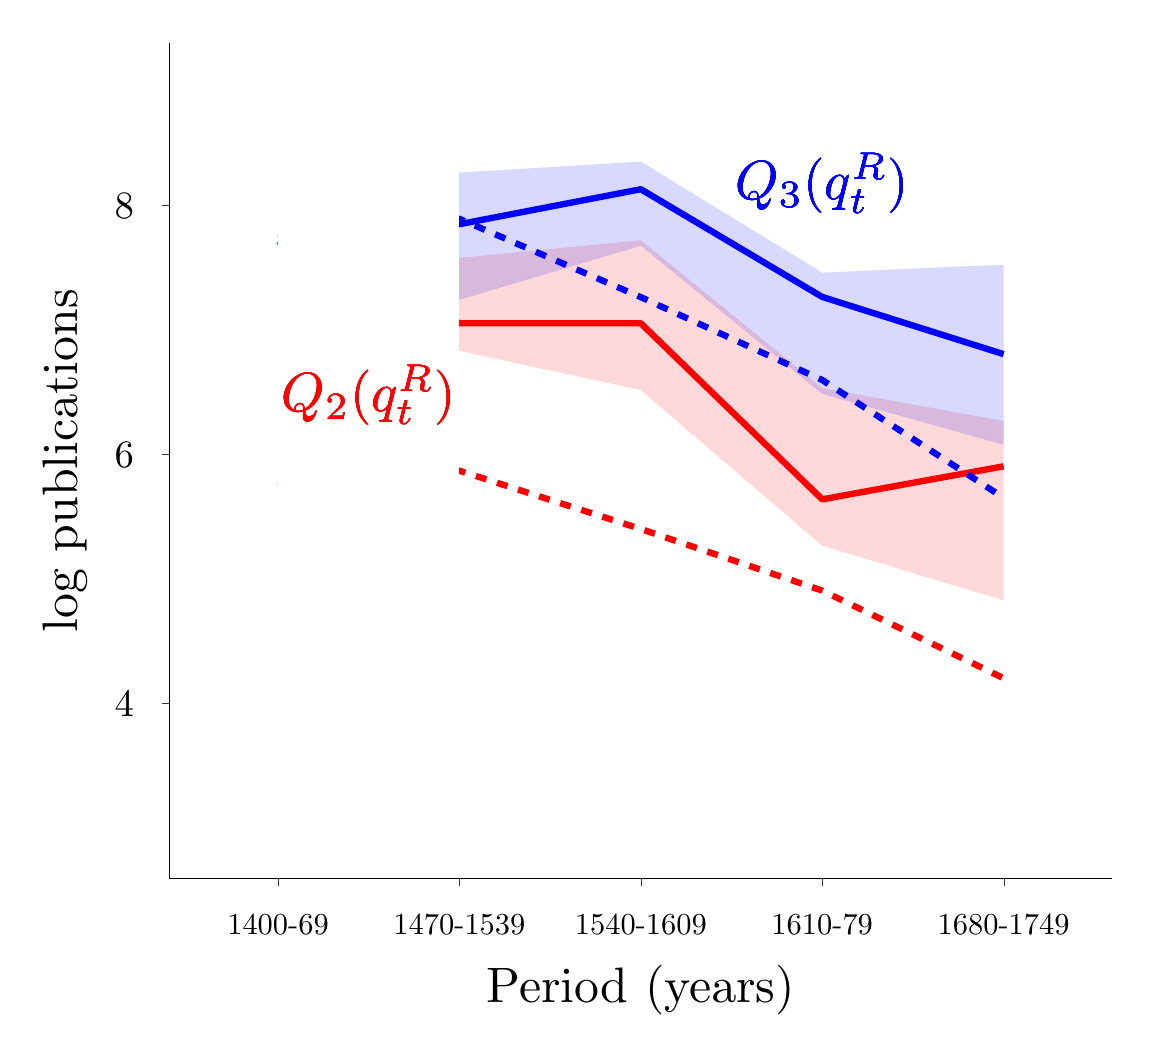
\begin{tikzpicture}[x=1pt,y=1pt]
\definecolor{fillColor}{RGB}{255,255,255}
\path[use as bounding box,fill=fillColor,fill opacity=0.00] (0,0) rectangle (397.48,361.35);
\begin{scope}
\path[clip] (  0.00,  0.00) rectangle (397.48,361.35);
\definecolor{drawColor}{RGB}{255,255,255}
\definecolor{fillColor}{RGB}{255,255,255}

\path[draw=drawColor,line width= 0.1pt,line join=round,line cap=round,fill=fillColor] (  0.00,  0.00) rectangle (397.48,361.35);
\end{scope}
\begin{scope}
\path[clip] ( 51.14, 53.86) rectangle (391.98,355.85);
\definecolor{fillColor}{RGB}{255,255,255}

\path[fill=fillColor] ( 51.14, 53.86) rectangle (391.98,355.85);
\definecolor{fillColor}{RGB}{255,0,0}

\path[fill=fillColor,fill opacity=0.15] ( 90.47,292.14) --
	(156.02,278.15) --
	(221.56,284.53) --
	(287.11,231.13) --
	(352.66,219.22) --
	(352.66,154.37) --
	(287.11,174.15) --
	(221.56,230.40) --
	(156.02,244.55) --
	( 90.47,254.76) --
	cycle;

\path[] ( 90.47,292.14) --
	(156.02,278.15) --
	(221.56,284.53) --
	(287.11,231.13) --
	(352.66,219.22);

\path[] (352.66,154.37) --
	(287.11,174.15) --
	(221.56,230.40) --
	(156.02,244.55) --
	( 90.47,254.76);
\definecolor{drawColor}{RGB}{255,0,0}

\path[draw=drawColor,line width= 2.3pt,line join=round] ( 90.47,284.23) --
	(156.02,254.56) --
	(221.56,254.52) --
	(287.11,190.91) --
	(352.66,202.85);

\path[draw=drawColor,line width= 2.3pt,dash pattern=on 4pt off 4pt ,line join=round] ( 90.47,195.87) --
	(156.02,201.25) --
	(221.56,180.20) --
	(287.11,157.93) --
	(352.66,126.27);
\definecolor{fillColor}{RGB}{0,0,255}

\path[fill=fillColor,fill opacity=0.15] ( 90.47,325.49) --
	(156.02,308.99) --
	(221.56,312.95) --
	(287.11,272.84) --
	(352.66,275.70) --
	(352.66,210.60) --
	(287.11,228.99) --
	(221.56,282.55) --
	(156.02,262.97) --
	( 90.47,278.47) --
	cycle;

\path[] ( 90.47,325.49) --
	(156.02,308.99) --
	(221.56,312.95) --
	(287.11,272.84) --
	(352.66,275.70);

\path[] (352.66,210.60) --
	(287.11,228.99) --
	(221.56,282.55) --
	(156.02,262.97) --
	( 90.47,278.47);
\definecolor{drawColor}{RGB}{0,0,255}

\path[draw=drawColor,line width= 2.3pt,line join=round] ( 90.47,291.49) --
	(156.02,290.33) --
	(221.56,302.97) --
	(287.11,264.05) --
	(352.66,243.37);

\path[draw=drawColor,line width= 2.3pt,dash pattern=on 4pt off 4pt ,line join=round] ( 90.47,285.04) --
	(156.02,292.27) --
	(221.56,263.97) --
	(287.11,234.03) --
	(352.66,191.46);
\definecolor{fillColor}{RGB}{255,255,255}

\path[fill=fillColor] ( 90.47, 53.86) rectangle (156.02,355.85);

\path[fill=fillColor] ( 90.47, 53.86) rectangle (156.02,355.85);

\path[fill=fillColor] ( 90.47, 53.86) rectangle (156.02,355.85);

\path[fill=fillColor] ( 90.47, 53.86) rectangle (156.02,355.85);

\path[fill=fillColor] ( 90.47, 53.86) rectangle (156.02,355.85);

\node[text=drawColor,anchor=base,inner sep=0pt, outer sep=0pt, scale=  1.99] at (287.11,299.26) {$Q_3(q_t^R)$};

\node[text=drawColor,anchor=base,inner sep=0pt, outer sep=0pt, scale=  1.99] at (287.11,299.26) {$Q_3(q_t^R)$};

\node[text=drawColor,anchor=base,inner sep=0pt, outer sep=0pt, scale=  1.99] at (287.11,299.26) {$Q_3(q_t^R)$};

\node[text=drawColor,anchor=base,inner sep=0pt, outer sep=0pt, scale=  1.99] at (287.11,299.26) {$Q_3(q_t^R)$};

\node[text=drawColor,anchor=base,inner sep=0pt, outer sep=0pt, scale=  1.99] at (287.11,299.26) {$Q_3(q_t^R)$};
\definecolor{drawColor}{RGB}{255,0,0}

\node[text=drawColor,anchor=base,inner sep=0pt, outer sep=0pt, scale=  1.99] at (123.25,222.75) {$Q_2(q_t^R)$};

\node[text=drawColor,anchor=base,inner sep=0pt, outer sep=0pt, scale=  1.99] at (123.25,222.75) {$Q_2(q_t^R)$};

\node[text=drawColor,anchor=base,inner sep=0pt, outer sep=0pt, scale=  1.99] at (123.25,222.75) {$Q_2(q_t^R)$};

\node[text=drawColor,anchor=base,inner sep=0pt, outer sep=0pt, scale=  1.99] at (123.25,222.75) {$Q_2(q_t^R)$};

\node[text=drawColor,anchor=base,inner sep=0pt, outer sep=0pt, scale=  1.99] at (123.25,222.75) {$Q_2(q_t^R)$};
\end{scope}
\begin{scope}
\path[clip] (  0.00,  0.00) rectangle (397.48,361.35);
\definecolor{drawColor}{RGB}{0,0,0}

\path[draw=drawColor,line width= 0.1pt,line join=round] ( 51.14, 53.86) --
	( 51.14,355.85);
\end{scope}
\begin{scope}
\path[clip] (  0.00,  0.00) rectangle (397.48,361.35);
\definecolor{drawColor}{RGB}{0,0,0}

\node[text=drawColor,anchor=base east,inner sep=0pt, outer sep=0pt, scale=  1.40] at ( 38.39,112.27) {4};

\node[text=drawColor,anchor=base east,inner sep=0pt, outer sep=0pt, scale=  1.40] at ( 38.39,202.28) {6};

\node[text=drawColor,anchor=base east,inner sep=0pt, outer sep=0pt, scale=  1.40] at ( 38.39,292.30) {8};
\end{scope}
\begin{scope}
\path[clip] (  0.00,  0.00) rectangle (397.48,361.35);
\definecolor{drawColor}{gray}{0.20}

\path[draw=drawColor,line width= 0.1pt,line join=round] ( 48.39,117.09) --
	( 51.14,117.09);

\path[draw=drawColor,line width= 0.1pt,line join=round] ( 48.39,207.11) --
	( 51.14,207.11);

\path[draw=drawColor,line width= 0.1pt,line join=round] ( 48.39,297.12) --
	( 51.14,297.12);
\end{scope}
\begin{scope}
\path[clip] (  0.00,  0.00) rectangle (397.48,361.35);
\definecolor{drawColor}{RGB}{0,0,0}

\path[draw=drawColor,line width= 0.1pt,line join=round] ( 51.14, 53.86) --
	(391.98, 53.86);
\end{scope}
\begin{scope}
\path[clip] (  0.00,  0.00) rectangle (397.48,361.35);
\definecolor{drawColor}{gray}{0.20}

\path[draw=drawColor,line width= 0.1pt,line join=round] ( 90.47, 51.11) --
	( 90.47, 53.86);

\path[draw=drawColor,line width= 0.1pt,line join=round] (156.02, 51.11) --
	(156.02, 53.86);

\path[draw=drawColor,line width= 0.1pt,line join=round] (221.56, 51.11) --
	(221.56, 53.86);

\path[draw=drawColor,line width= 0.1pt,line join=round] (287.11, 51.11) --
	(287.11, 53.86);

\path[draw=drawColor,line width= 0.1pt,line join=round] (352.66, 51.11) --
	(352.66, 53.86);
\end{scope}
\begin{scope}
\path[clip] (  0.00,  0.00) rectangle (397.48,361.35);
\definecolor{drawColor}{RGB}{0,0,0}

\node[text=drawColor,anchor=base,inner sep=0pt, outer sep=0pt, scale=  1.10] at ( 90.47, 33.53) {1400-69};

\node[text=drawColor,anchor=base,inner sep=0pt, outer sep=0pt, scale=  1.10] at (156.02, 33.53) {1470-1539};

\node[text=drawColor,anchor=base,inner sep=0pt, outer sep=0pt, scale=  1.10] at (221.56, 33.53) {1540-1609};

\node[text=drawColor,anchor=base,inner sep=0pt, outer sep=0pt, scale=  1.10] at (287.11, 33.53) {1610-79};

\node[text=drawColor,anchor=base,inner sep=0pt, outer sep=0pt, scale=  1.10] at (352.66, 33.53) {1680-1749};
\end{scope}
\begin{scope}
\path[clip] (  0.00,  0.00) rectangle (397.48,361.35);
\definecolor{drawColor}{RGB}{0,0,0}

\node[text=drawColor,anchor=base,inner sep=0pt, outer sep=0pt, scale=  1.80] at (221.56,  9.00) {Period (years)};
\end{scope}
\begin{scope}
\path[clip] (  0.00,  0.00) rectangle (397.48,361.35);
\definecolor{drawColor}{RGB}{0,0,0}

\node[text=drawColor,rotate= 90.00,anchor=base,inner sep=0pt, outer sep=0pt, scale=  1.80] at ( 17.90,204.86) {log publications};
\end{scope}
\end{tikzpicture}
 }
}
\parbox{.49\textwidth}{
		\centering
{Non-censored scholars\\
quality: \textcolor{red}{median}, \textcolor{blue}{$75^{th}$ percentile}}

\scalebox{0.45}{% Created by tikzDevice version 0.12.3.1 on 2022-09-19 22:27:53
% !TEX encoding = UTF-8 Unicode
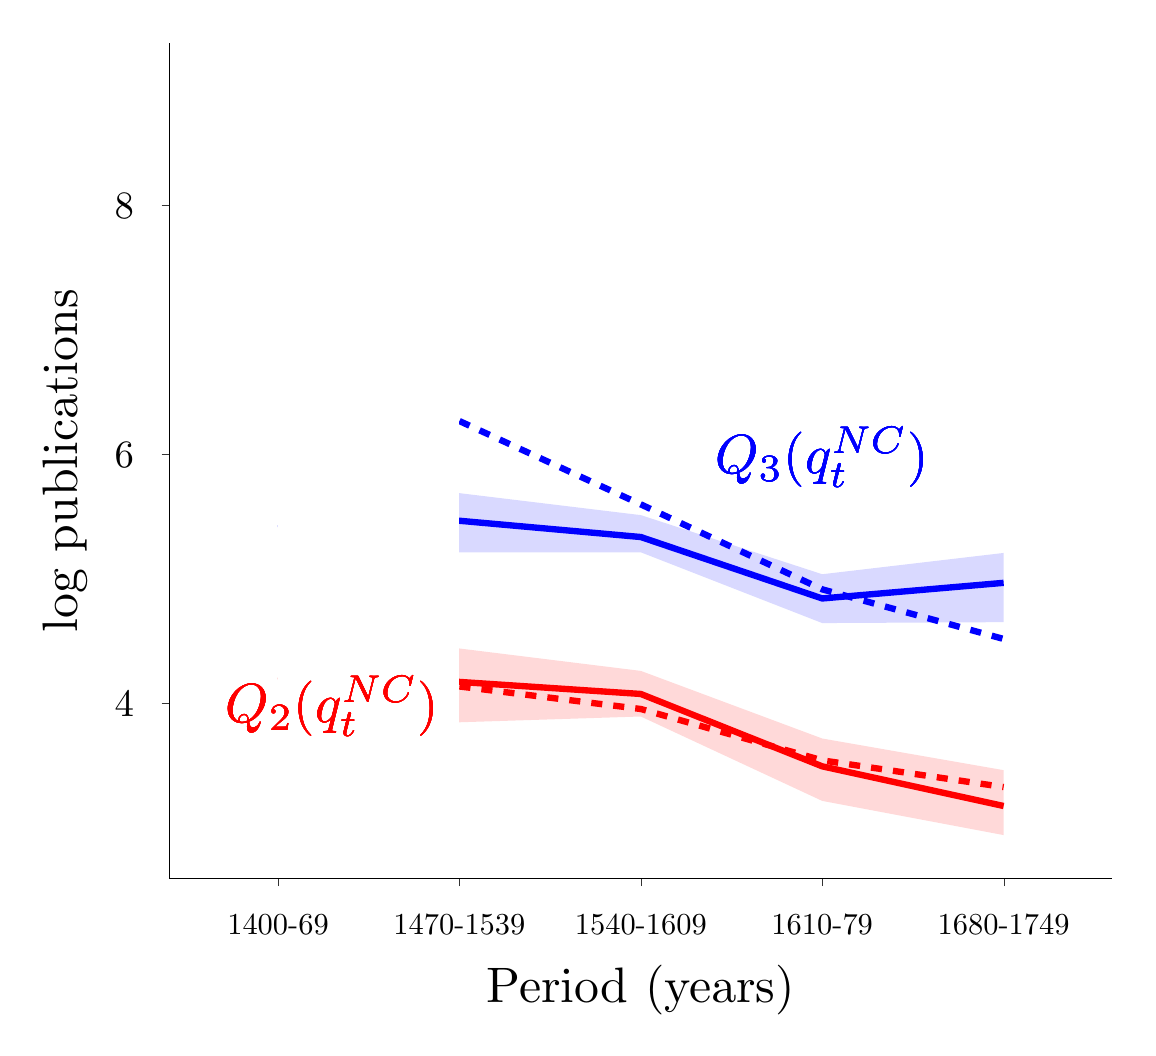
\begin{tikzpicture}[x=1pt,y=1pt]
\definecolor{fillColor}{RGB}{255,255,255}
\path[use as bounding box,fill=fillColor,fill opacity=0.00] (0,0) rectangle (397.48,361.35);
\begin{scope}
\path[clip] (  0.00,  0.00) rectangle (397.48,361.35);
\definecolor{drawColor}{RGB}{255,255,255}
\definecolor{fillColor}{RGB}{255,255,255}

\path[draw=drawColor,line width= 0.1pt,line join=round,line cap=round,fill=fillColor] (  0.00,  0.00) rectangle (397.48,361.35);
\end{scope}
\begin{scope}
\path[clip] ( 51.14, 53.86) rectangle (391.98,355.85);
\definecolor{fillColor}{RGB}{255,255,255}

\path[fill=fillColor] ( 51.14, 53.86) rectangle (391.98,355.85);
\definecolor{fillColor}{RGB}{255,0,0}

\path[fill=fillColor,fill opacity=0.15] ( 90.47,136.22) --
	(156.02,137.02) --
	(221.56,128.92) --
	(287.11,104.49) --
	(352.66, 93.05) --
	(352.66, 69.59) --
	(287.11, 81.94) --
	(221.56,112.44) --
	(156.02,110.35) --
	( 90.47,106.78) --
	cycle;

\path[] ( 90.47,136.22) --
	(156.02,137.02) --
	(221.56,128.92) --
	(287.11,104.49) --
	(352.66, 93.05);

\path[] (352.66, 69.59) --
	(287.11, 81.94) --
	(221.56,112.44) --
	(156.02,110.35) --
	( 90.47,106.78);
\definecolor{drawColor}{RGB}{255,0,0}

\path[draw=drawColor,line width= 2.3pt,line join=round] ( 90.47,126.97) --
	(156.02,124.94) --
	(221.56,120.58) --
	(287.11, 94.43) --
	(352.66, 80.10);

\path[draw=drawColor,line width= 2.3pt,dash pattern=on 4pt off 4pt ,line join=round] (156.02,123.30) --
	(221.56,115.15) --
	(287.11, 96.59) --
	(352.66, 86.95);
\definecolor{fillColor}{RGB}{0,0,255}

\path[fill=fillColor,fill opacity=0.15] ( 90.47,199.10) --
	(156.02,193.15) --
	(221.56,185.21) --
	(287.11,163.85) --
	(352.66,171.54) --
	(352.66,146.53) --
	(287.11,146.20) --
	(221.56,171.77) --
	(156.02,171.76) --
	( 90.47,164.34) --
	cycle;

\path[] ( 90.47,199.10) --
	(156.02,193.15) --
	(221.56,185.21) --
	(287.11,163.85) --
	(352.66,171.54);

\path[] (352.66,146.53) --
	(287.11,146.20) --
	(221.56,171.77) --
	(156.02,171.76) --
	( 90.47,164.34);
\definecolor{drawColor}{RGB}{0,0,255}

\path[draw=drawColor,line width= 2.3pt,line join=round] ( 90.47,180.48) --
	(156.02,183.17) --
	(221.56,177.29) --
	(287.11,155.09) --
	(352.66,160.74);

\path[draw=drawColor,line width= 2.3pt,dash pattern=on 4pt off 4pt ,line join=round] (156.02,219.20) --
	(221.56,189.09) --
	(287.11,158.39) --
	(352.66,140.46);
\definecolor{fillColor}{RGB}{255,255,255}

\path[fill=fillColor] ( 90.47, 53.86) rectangle (156.02,355.85);

\path[fill=fillColor] ( 90.47, 53.86) rectangle (156.02,355.85);

\path[fill=fillColor] ( 90.47, 53.86) rectangle (156.02,355.85);

\path[fill=fillColor] ( 90.47, 53.86) rectangle (156.02,355.85);

\path[fill=fillColor] ( 90.47, 53.86) rectangle (156.02,355.85);

\node[text=drawColor,anchor=base,inner sep=0pt, outer sep=0pt, scale=  1.99] at (287.11,200.25) {$Q_3(q_t^{NC})$};

\node[text=drawColor,anchor=base,inner sep=0pt, outer sep=0pt, scale=  1.99] at (287.11,200.25) {$Q_3(q_t^{NC})$};

\node[text=drawColor,anchor=base,inner sep=0pt, outer sep=0pt, scale=  1.99] at (287.11,200.25) {$Q_3(q_t^{NC})$};

\node[text=drawColor,anchor=base,inner sep=0pt, outer sep=0pt, scale=  1.99] at (287.11,200.25) {$Q_3(q_t^{NC})$};

\node[text=drawColor,anchor=base,inner sep=0pt, outer sep=0pt, scale=  1.99] at (287.11,200.25) {$Q_3(q_t^{NC})$};
\definecolor{drawColor}{RGB}{255,0,0}

\node[text=drawColor,anchor=base,inner sep=0pt, outer sep=0pt, scale=  1.99] at (110.14,110.23) {$Q_2(q_t^{NC})$};

\node[text=drawColor,anchor=base,inner sep=0pt, outer sep=0pt, scale=  1.99] at (110.14,110.23) {$Q_2(q_t^{NC})$};

\node[text=drawColor,anchor=base,inner sep=0pt, outer sep=0pt, scale=  1.99] at (110.14,110.23) {$Q_2(q_t^{NC})$};

\node[text=drawColor,anchor=base,inner sep=0pt, outer sep=0pt, scale=  1.99] at (110.14,110.23) {$Q_2(q_t^{NC})$};

\node[text=drawColor,anchor=base,inner sep=0pt, outer sep=0pt, scale=  1.99] at (110.14,110.23) {$Q_2(q_t^{NC})$};
\end{scope}
\begin{scope}
\path[clip] (  0.00,  0.00) rectangle (397.48,361.35);
\definecolor{drawColor}{RGB}{0,0,0}

\path[draw=drawColor,line width= 0.1pt,line join=round] ( 51.14, 53.86) --
	( 51.14,355.85);
\end{scope}
\begin{scope}
\path[clip] (  0.00,  0.00) rectangle (397.48,361.35);
\definecolor{drawColor}{RGB}{0,0,0}

\node[text=drawColor,anchor=base east,inner sep=0pt, outer sep=0pt, scale=  1.40] at ( 38.39,112.27) {4};

\node[text=drawColor,anchor=base east,inner sep=0pt, outer sep=0pt, scale=  1.40] at ( 38.39,202.28) {6};

\node[text=drawColor,anchor=base east,inner sep=0pt, outer sep=0pt, scale=  1.40] at ( 38.39,292.30) {8};
\end{scope}
\begin{scope}
\path[clip] (  0.00,  0.00) rectangle (397.48,361.35);
\definecolor{drawColor}{gray}{0.20}

\path[draw=drawColor,line width= 0.1pt,line join=round] ( 48.39,117.09) --
	( 51.14,117.09);

\path[draw=drawColor,line width= 0.1pt,line join=round] ( 48.39,207.11) --
	( 51.14,207.11);

\path[draw=drawColor,line width= 0.1pt,line join=round] ( 48.39,297.12) --
	( 51.14,297.12);
\end{scope}
\begin{scope}
\path[clip] (  0.00,  0.00) rectangle (397.48,361.35);
\definecolor{drawColor}{RGB}{0,0,0}

\path[draw=drawColor,line width= 0.1pt,line join=round] ( 51.14, 53.86) --
	(391.98, 53.86);
\end{scope}
\begin{scope}
\path[clip] (  0.00,  0.00) rectangle (397.48,361.35);
\definecolor{drawColor}{gray}{0.20}

\path[draw=drawColor,line width= 0.1pt,line join=round] ( 90.47, 51.11) --
	( 90.47, 53.86);

\path[draw=drawColor,line width= 0.1pt,line join=round] (156.02, 51.11) --
	(156.02, 53.86);

\path[draw=drawColor,line width= 0.1pt,line join=round] (221.56, 51.11) --
	(221.56, 53.86);

\path[draw=drawColor,line width= 0.1pt,line join=round] (287.11, 51.11) --
	(287.11, 53.86);

\path[draw=drawColor,line width= 0.1pt,line join=round] (352.66, 51.11) --
	(352.66, 53.86);
\end{scope}
\begin{scope}
\path[clip] (  0.00,  0.00) rectangle (397.48,361.35);
\definecolor{drawColor}{RGB}{0,0,0}

\node[text=drawColor,anchor=base,inner sep=0pt, outer sep=0pt, scale=  1.10] at ( 90.47, 33.53) {1400-69};

\node[text=drawColor,anchor=base,inner sep=0pt, outer sep=0pt, scale=  1.10] at (156.02, 33.53) {1470-1539};

\node[text=drawColor,anchor=base,inner sep=0pt, outer sep=0pt, scale=  1.10] at (221.56, 33.53) {1540-1609};

\node[text=drawColor,anchor=base,inner sep=0pt, outer sep=0pt, scale=  1.10] at (287.11, 33.53) {1610-79};

\node[text=drawColor,anchor=base,inner sep=0pt, outer sep=0pt, scale=  1.10] at (352.66, 33.53) {1680-1749};
\end{scope}
\begin{scope}
\path[clip] (  0.00,  0.00) rectangle (397.48,361.35);
\definecolor{drawColor}{RGB}{0,0,0}

\node[text=drawColor,anchor=base,inner sep=0pt, outer sep=0pt, scale=  1.80] at (221.56,  9.00) {Period (years)};
\end{scope}
\begin{scope}
\path[clip] (  0.00,  0.00) rectangle (397.48,361.35);
\definecolor{drawColor}{RGB}{0,0,0}

\node[text=drawColor,rotate= 90.00,anchor=base,inner sep=0pt, outer sep=0pt, scale=  1.80] at ( 17.90,204.86) {log publications};
\end{scope}
\end{tikzpicture}
}
}

 \end{frame}


%%%%%%%%%%%%%%%%%%%%%%%%%%%%%%%%%%%%%%%%%%%%%%%%%%%%%%%%%%%%%%%%%%%%%%%%%%%%%%%%%%%%%%%%%%%%%%%%%%%%%%%%%%%%%%%%%%%%%%%%%%%%%%%%%%%%%%%%%%%%%%%%%%%%%%%
	\section{Simulation}
	\subsection{}

	\begin{frame}
\frametitle{With and without censorship}

\begin{figure}
	\begin{subfigure}{.32\textwidth}
		\centering
		% include second image
		\caption{\% censored authors\\\textcolor{white}{a}}
		\label{sf:ca}
		\scalebox{0.34}{% Created by tikzDevice version 0.12.3.1 on 2022-09-19 21:45:17
% !TEX encoding = UTF-8 Unicode
\begin{tikzpicture}[x=1pt,y=1pt]
\definecolor{fillColor}{RGB}{255,255,255}
\path[use as bounding box,fill=fillColor,fill opacity=0.00] (0,0) rectangle (397.48,289.08);
\begin{scope}
\path[clip] (  0.00,  0.00) rectangle (397.48,289.08);
\definecolor{drawColor}{RGB}{255,255,255}
\definecolor{fillColor}{RGB}{255,255,255}

\path[draw=drawColor,line width= 0.1pt,line join=round,line cap=round,fill=fillColor] (  0.00,  0.00) rectangle (397.48,289.08);
\end{scope}
\begin{scope}
\path[clip] ( 51.14, 53.86) rectangle (391.98,283.58);
\definecolor{fillColor}{RGB}{255,255,255}

\path[fill=fillColor] ( 51.14, 53.86) rectangle (391.98,283.58);
\definecolor{drawColor}{RGB}{169,169,169}

\path[draw=drawColor,line width= 2.3pt,line join=round] ( 90.47,271.50) --
	(156.02,273.14) --
	(221.56,255.25) --
	(287.11,220.38) --
	(352.66,160.32);

\path[draw=drawColor,line width= 2.3pt,dash pattern=on 4pt off 4pt ,line join=round] ( 90.47, 64.30) --
	(156.02, 64.30) --
	(221.56, 64.30) --
	(287.11, 64.30) --
	(352.66, 64.30);

\path[fill=fillColor] ( 90.47, 53.86) rectangle (156.02,283.58);

\path[fill=fillColor] ( 90.47, 53.86) rectangle (156.02,283.58);

\path[fill=fillColor] ( 90.47, 53.86) rectangle (156.02,283.58);

\path[fill=fillColor] ( 90.47, 53.86) rectangle (156.02,283.58);

\path[fill=fillColor] ( 90.47, 53.86) rectangle (156.02,283.58);
\end{scope}
\begin{scope}
\path[clip] (  0.00,  0.00) rectangle (397.48,289.08);
\definecolor{drawColor}{RGB}{0,0,0}

\path[draw=drawColor,line width= 0.1pt,line join=round] ( 51.14, 53.86) --
	( 51.14,283.58);
\end{scope}
\begin{scope}
\path[clip] (  0.00,  0.00) rectangle (397.48,289.08);
\definecolor{drawColor}{RGB}{0,0,0}

\node[text=drawColor,anchor=base east,inner sep=0pt, outer sep=0pt, scale=  1.40] at ( 38.39,147.78) {4};

\node[text=drawColor,anchor=base east,inner sep=0pt, outer sep=0pt, scale=  1.40] at ( 38.39,236.08) {8};
\end{scope}
\begin{scope}
\path[clip] (  0.00,  0.00) rectangle (397.48,289.08);
\definecolor{drawColor}{gray}{0.20}

\path[draw=drawColor,line width= 0.1pt,line join=round] ( 48.39,152.60) --
	( 51.14,152.60);

\path[draw=drawColor,line width= 0.1pt,line join=round] ( 48.39,240.90) --
	( 51.14,240.90);
\end{scope}
\begin{scope}
\path[clip] (  0.00,  0.00) rectangle (397.48,289.08);
\definecolor{drawColor}{RGB}{0,0,0}

\path[draw=drawColor,line width= 0.1pt,line join=round] ( 51.14, 53.86) --
	(391.98, 53.86);
\end{scope}
\begin{scope}
\path[clip] (  0.00,  0.00) rectangle (397.48,289.08);
\definecolor{drawColor}{gray}{0.20}

\path[draw=drawColor,line width= 0.1pt,line join=round] ( 90.47, 51.11) --
	( 90.47, 53.86);

\path[draw=drawColor,line width= 0.1pt,line join=round] (156.02, 51.11) --
	(156.02, 53.86);

\path[draw=drawColor,line width= 0.1pt,line join=round] (221.56, 51.11) --
	(221.56, 53.86);

\path[draw=drawColor,line width= 0.1pt,line join=round] (287.11, 51.11) --
	(287.11, 53.86);

\path[draw=drawColor,line width= 0.1pt,line join=round] (352.66, 51.11) --
	(352.66, 53.86);
\end{scope}
\begin{scope}
\path[clip] (  0.00,  0.00) rectangle (397.48,289.08);
\definecolor{drawColor}{RGB}{0,0,0}

\node[text=drawColor,anchor=base,inner sep=0pt, outer sep=0pt, scale=  1.10] at ( 90.47, 33.53) {1400-69};

\node[text=drawColor,anchor=base,inner sep=0pt, outer sep=0pt, scale=  1.10] at (156.02, 33.53) {1470-1539};

\node[text=drawColor,anchor=base,inner sep=0pt, outer sep=0pt, scale=  1.10] at (221.56, 33.53) {1540-1609};

\node[text=drawColor,anchor=base,inner sep=0pt, outer sep=0pt, scale=  1.10] at (287.11, 33.53) {1610-79};

\node[text=drawColor,anchor=base,inner sep=0pt, outer sep=0pt, scale=  1.10] at (352.66, 33.53) {1680-1749};
\end{scope}
\begin{scope}
\path[clip] (  0.00,  0.00) rectangle (397.48,289.08);
\definecolor{drawColor}{RGB}{0,0,0}

\node[text=drawColor,anchor=base,inner sep=0pt, outer sep=0pt, scale=  1.80] at (221.56,  9.00) {Period (years)};
\end{scope}
\begin{scope}
\path[clip] (  0.00,  0.00) rectangle (397.48,289.08);
\definecolor{drawColor}{RGB}{0,0,0}

\node[text=drawColor,rotate= 90.00,anchor=base,inner sep=0pt, outer sep=0pt, scale=  1.80] at ( 17.90,168.72) {$\overline{\beta}m_t$ (\%) };
\end{scope}
\end{tikzpicture}
 }
	\end{subfigure}
	\begin{subfigure}{.32\textwidth}
		\centering
		% include first image
		\caption{\% revolutionary authors\\\textcolor{white}{a}}
		\label{sf:ra}
		\scalebox{0.34}{% Created by tikzDevice version 0.12.3.1 on 2022-09-19 22:27:55
% !TEX encoding = UTF-8 Unicode
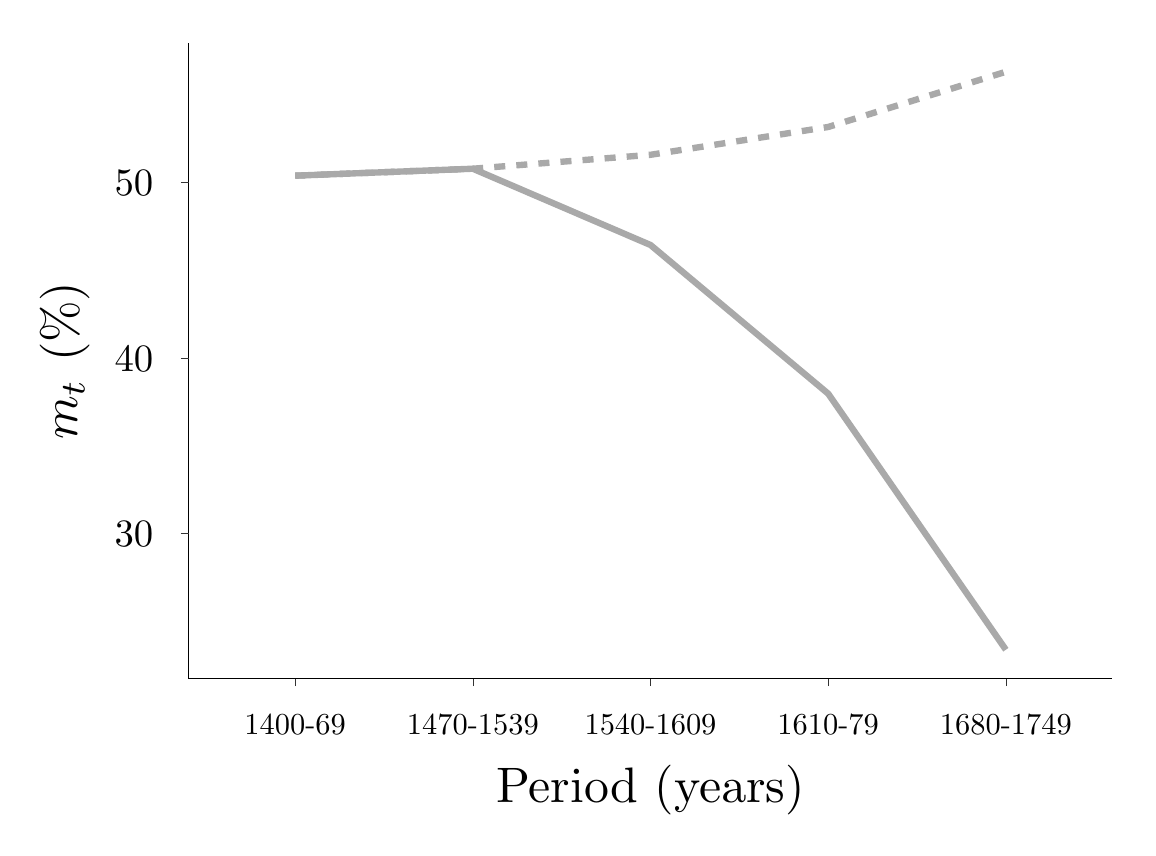
\begin{tikzpicture}[x=1pt,y=1pt]
\definecolor{fillColor}{RGB}{255,255,255}
\path[use as bounding box,fill=fillColor,fill opacity=0.00] (0,0) rectangle (397.48,289.08);
\begin{scope}
\path[clip] (  0.00,  0.00) rectangle (397.48,289.08);
\definecolor{drawColor}{RGB}{255,255,255}
\definecolor{fillColor}{RGB}{255,255,255}

\path[draw=drawColor,line width= 0.1pt,line join=round,line cap=round,fill=fillColor] (  0.00,  0.00) rectangle (397.48,289.08);
\end{scope}
\begin{scope}
\path[clip] ( 58.14, 53.86) rectangle (391.98,283.58);
\definecolor{fillColor}{RGB}{255,255,255}

\path[fill=fillColor] ( 58.14, 53.86) rectangle (391.98,283.58);
\definecolor{drawColor}{RGB}{169,169,169}

\path[draw=drawColor,line width= 2.3pt,line join=round] ( 96.66,235.59) --
	(160.86,238.11) --
	(225.06,210.55) --
	(289.26,156.83) --
	(353.46, 64.30);

\path[draw=drawColor,line width= 2.3pt,dash pattern=on 4pt off 4pt ,line join=round] ( 96.66,235.59) --
	(160.86,238.11) --
	(225.06,243.14) --
	(289.26,253.19) --
	(353.46,273.14);
\end{scope}
\begin{scope}
\path[clip] (  0.00,  0.00) rectangle (397.48,289.08);
\definecolor{drawColor}{RGB}{0,0,0}

\path[draw=drawColor,line width= 0.1pt,line join=round] ( 58.14, 53.86) --
	( 58.14,283.58);
\end{scope}
\begin{scope}
\path[clip] (  0.00,  0.00) rectangle (397.48,289.08);
\definecolor{drawColor}{RGB}{0,0,0}

\node[text=drawColor,anchor=base east,inner sep=0pt, outer sep=0pt, scale=  1.40] at ( 45.39,101.57) {30};

\node[text=drawColor,anchor=base east,inner sep=0pt, outer sep=0pt, scale=  1.40] at ( 45.39,164.91) {40};

\node[text=drawColor,anchor=base east,inner sep=0pt, outer sep=0pt, scale=  1.40] at ( 45.39,228.26) {50};
\end{scope}
\begin{scope}
\path[clip] (  0.00,  0.00) rectangle (397.48,289.08);
\definecolor{drawColor}{gray}{0.20}

\path[draw=drawColor,line width= 0.1pt,line join=round] ( 55.39,106.39) --
	( 58.14,106.39);

\path[draw=drawColor,line width= 0.1pt,line join=round] ( 55.39,169.73) --
	( 58.14,169.73);

\path[draw=drawColor,line width= 0.1pt,line join=round] ( 55.39,233.08) --
	( 58.14,233.08);
\end{scope}
\begin{scope}
\path[clip] (  0.00,  0.00) rectangle (397.48,289.08);
\definecolor{drawColor}{RGB}{0,0,0}

\path[draw=drawColor,line width= 0.1pt,line join=round] ( 58.14, 53.86) --
	(391.98, 53.86);
\end{scope}
\begin{scope}
\path[clip] (  0.00,  0.00) rectangle (397.48,289.08);
\definecolor{drawColor}{gray}{0.20}

\path[draw=drawColor,line width= 0.1pt,line join=round] ( 96.66, 51.11) --
	( 96.66, 53.86);

\path[draw=drawColor,line width= 0.1pt,line join=round] (160.86, 51.11) --
	(160.86, 53.86);

\path[draw=drawColor,line width= 0.1pt,line join=round] (225.06, 51.11) --
	(225.06, 53.86);

\path[draw=drawColor,line width= 0.1pt,line join=round] (289.26, 51.11) --
	(289.26, 53.86);

\path[draw=drawColor,line width= 0.1pt,line join=round] (353.46, 51.11) --
	(353.46, 53.86);
\end{scope}
\begin{scope}
\path[clip] (  0.00,  0.00) rectangle (397.48,289.08);
\definecolor{drawColor}{RGB}{0,0,0}

\node[text=drawColor,anchor=base,inner sep=0pt, outer sep=0pt, scale=  1.10] at ( 96.66, 33.53) {1400-69};

\node[text=drawColor,anchor=base,inner sep=0pt, outer sep=0pt, scale=  1.10] at (160.86, 33.53) {1470-1539};

\node[text=drawColor,anchor=base,inner sep=0pt, outer sep=0pt, scale=  1.10] at (225.06, 33.53) {1540-1609};

\node[text=drawColor,anchor=base,inner sep=0pt, outer sep=0pt, scale=  1.10] at (289.26, 33.53) {1610-79};

\node[text=drawColor,anchor=base,inner sep=0pt, outer sep=0pt, scale=  1.10] at (353.46, 33.53) {1680-1749};
\end{scope}
\begin{scope}
\path[clip] (  0.00,  0.00) rectangle (397.48,289.08);
\definecolor{drawColor}{RGB}{0,0,0}

\node[text=drawColor,anchor=base,inner sep=0pt, outer sep=0pt, scale=  1.80] at (225.06,  9.00) {Period (years)};
\end{scope}
\begin{scope}
\path[clip] (  0.00,  0.00) rectangle (397.48,289.08);
\definecolor{drawColor}{RGB}{0,0,0}

\node[text=drawColor,rotate= 90.00,anchor=base,inner sep=0pt, outer sep=0pt, scale=  1.80] at ( 17.90,168.72) {$m_t$ (\%)};
\end{scope}
\end{tikzpicture}
 }
	\end{subfigure}
	\begin{subfigure}{.32\textwidth}
		\centering
		% include second image
		\caption{\textcolor{blue}{Overall}, \textcolor{red}{revolutionary}\\ \textcolor{orange}{compliant} quality (averages)}
		\label{sf:dq}
		\scalebox{0.34}{% Created by tikzDevice version 0.12.3.1 on 2022-09-19 22:27:55
% !TEX encoding = UTF-8 Unicode
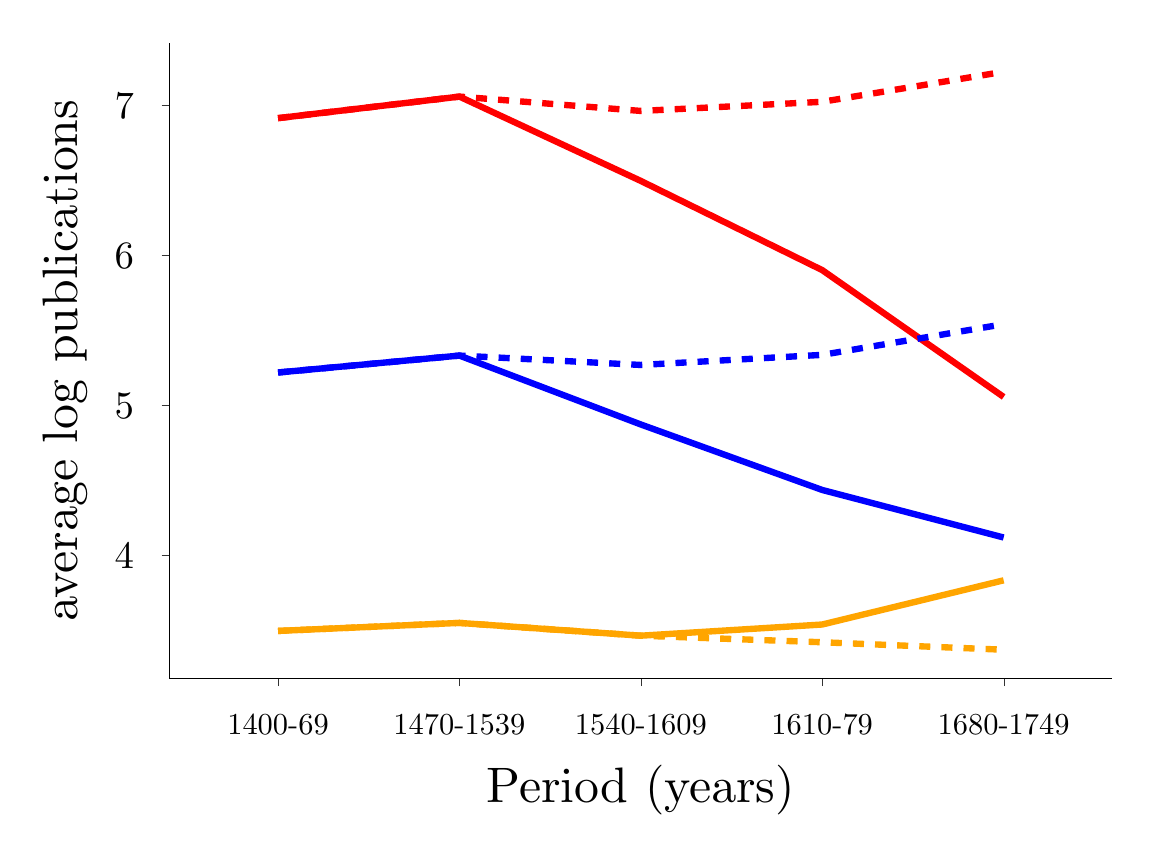
\begin{tikzpicture}[x=1pt,y=1pt]
\definecolor{fillColor}{RGB}{255,255,255}
\path[use as bounding box,fill=fillColor,fill opacity=0.00] (0,0) rectangle (397.48,289.08);
\begin{scope}
\path[clip] (  0.00,  0.00) rectangle (397.48,289.08);
\definecolor{drawColor}{RGB}{255,255,255}
\definecolor{fillColor}{RGB}{255,255,255}

\path[draw=drawColor,line width= 0.1pt,line join=round,line cap=round,fill=fillColor] (  0.00,  0.00) rectangle (397.48,289.08);
\end{scope}
\begin{scope}
\path[clip] ( 51.14, 53.86) rectangle (391.98,283.58);
\definecolor{fillColor}{RGB}{255,255,255}

\path[fill=fillColor] ( 51.14, 53.86) rectangle (391.98,283.58);
\definecolor{drawColor}{RGB}{255,0,0}

\path[draw=drawColor,line width= 2.3pt,line join=round] ( 90.47,256.38) --
	(156.02,264.17) --
	(221.56,233.70) --
	(287.11,201.47) --
	(352.66,155.64);

\path[draw=drawColor,line width= 2.3pt,dash pattern=on 4pt off 4pt ,line join=round] ( 90.47,256.38) --
	(156.02,264.17) --
	(221.56,258.99) --
	(287.11,262.29) --
	(352.66,273.14);
\definecolor{drawColor}{RGB}{0,0,255}

\path[draw=drawColor,line width= 2.3pt,line join=round] ( 90.47,164.47) --
	(156.02,170.59) --
	(221.56,145.69) --
	(287.11,122.03) --
	(352.66,104.85);

\path[draw=drawColor,line width= 2.3pt,dash pattern=on 4pt off 4pt ,line join=round] ( 90.47,164.47) --
	(156.02,170.59) --
	(221.56,167.20) --
	(287.11,170.85) --
	(352.66,181.93);
\definecolor{drawColor}{RGB}{255,165,0}

\path[draw=drawColor,line width= 2.3pt,line join=round] ( 90.47, 71.09) --
	(156.02, 73.99) --
	(221.56, 69.37) --
	(287.11, 73.41) --
	(352.66, 89.38);

\path[draw=drawColor,line width= 2.3pt,dash pattern=on 4pt off 4pt ,line join=round] ( 90.47, 71.09) --
	(156.02, 73.99) --
	(221.56, 69.37) --
	(287.11, 67.00) --
	(352.66, 64.30);
\end{scope}
\begin{scope}
\path[clip] (  0.00,  0.00) rectangle (397.48,289.08);
\definecolor{drawColor}{RGB}{0,0,0}

\path[draw=drawColor,line width= 0.1pt,line join=round] ( 51.14, 53.86) --
	( 51.14,283.58);
\end{scope}
\begin{scope}
\path[clip] (  0.00,  0.00) rectangle (397.48,289.08);
\definecolor{drawColor}{RGB}{0,0,0}

\node[text=drawColor,anchor=base east,inner sep=0pt, outer sep=0pt, scale=  1.40] at ( 38.39, 93.70) {4};

\node[text=drawColor,anchor=base east,inner sep=0pt, outer sep=0pt, scale=  1.40] at ( 38.39,147.89) {5};

\node[text=drawColor,anchor=base east,inner sep=0pt, outer sep=0pt, scale=  1.40] at ( 38.39,202.08) {6};

\node[text=drawColor,anchor=base east,inner sep=0pt, outer sep=0pt, scale=  1.40] at ( 38.39,256.27) {7};
\end{scope}
\begin{scope}
\path[clip] (  0.00,  0.00) rectangle (397.48,289.08);
\definecolor{drawColor}{gray}{0.20}

\path[draw=drawColor,line width= 0.1pt,line join=round] ( 48.39, 98.52) --
	( 51.14, 98.52);

\path[draw=drawColor,line width= 0.1pt,line join=round] ( 48.39,152.71) --
	( 51.14,152.71);

\path[draw=drawColor,line width= 0.1pt,line join=round] ( 48.39,206.90) --
	( 51.14,206.90);

\path[draw=drawColor,line width= 0.1pt,line join=round] ( 48.39,261.09) --
	( 51.14,261.09);
\end{scope}
\begin{scope}
\path[clip] (  0.00,  0.00) rectangle (397.48,289.08);
\definecolor{drawColor}{RGB}{0,0,0}

\path[draw=drawColor,line width= 0.1pt,line join=round] ( 51.14, 53.86) --
	(391.98, 53.86);
\end{scope}
\begin{scope}
\path[clip] (  0.00,  0.00) rectangle (397.48,289.08);
\definecolor{drawColor}{gray}{0.20}

\path[draw=drawColor,line width= 0.1pt,line join=round] ( 90.47, 51.11) --
	( 90.47, 53.86);

\path[draw=drawColor,line width= 0.1pt,line join=round] (156.02, 51.11) --
	(156.02, 53.86);

\path[draw=drawColor,line width= 0.1pt,line join=round] (221.56, 51.11) --
	(221.56, 53.86);

\path[draw=drawColor,line width= 0.1pt,line join=round] (287.11, 51.11) --
	(287.11, 53.86);

\path[draw=drawColor,line width= 0.1pt,line join=round] (352.66, 51.11) --
	(352.66, 53.86);
\end{scope}
\begin{scope}
\path[clip] (  0.00,  0.00) rectangle (397.48,289.08);
\definecolor{drawColor}{RGB}{0,0,0}

\node[text=drawColor,anchor=base,inner sep=0pt, outer sep=0pt, scale=  1.10] at ( 90.47, 33.53) {1400-69};

\node[text=drawColor,anchor=base,inner sep=0pt, outer sep=0pt, scale=  1.10] at (156.02, 33.53) {1470-1539};

\node[text=drawColor,anchor=base,inner sep=0pt, outer sep=0pt, scale=  1.10] at (221.56, 33.53) {1540-1609};

\node[text=drawColor,anchor=base,inner sep=0pt, outer sep=0pt, scale=  1.10] at (287.11, 33.53) {1610-79};

\node[text=drawColor,anchor=base,inner sep=0pt, outer sep=0pt, scale=  1.10] at (352.66, 33.53) {1680-1749};
\end{scope}
\begin{scope}
\path[clip] (  0.00,  0.00) rectangle (397.48,289.08);
\definecolor{drawColor}{RGB}{0,0,0}

\node[text=drawColor,anchor=base,inner sep=0pt, outer sep=0pt, scale=  1.80] at (221.56,  9.00) {Period (years)};
\end{scope}
\begin{scope}
\path[clip] (  0.00,  0.00) rectangle (397.48,289.08);
\definecolor{drawColor}{RGB}{0,0,0}

\node[text=drawColor,rotate= 90.00,anchor=base,inner sep=0pt, outer sep=0pt, scale=  1.80] at ( 17.90,168.72) {average log publications};
\end{scope}
\end{tikzpicture}
 }
	\end{subfigure}

\end{figure}

 \end{frame}

 	\begin{frame}
\frametitle{Decomposition of effect of censorship}

 The loss in  the overall quality is  driven both by a reduction in the stock of available knowledge  and by the distortion in occupational choice:
\begin{equation}\label{eq:deco}
\begin{split}
\underbrace{q_5-\hat{q}_5}_{\text{=$-$1.41 (100\%)}}=&\underbrace{\hat{m}_5 [{q}^R_5-\hat{q}^R_5]+(1-\hat{m}_5)[q^C_5-\hat{q}^C_5]}_{\text{=$-$1.03 (72\%); $(a)$}}+\\&\underbrace{[m_5-\hat{m_5}]\hat{q}^R_5+[(1-m_5)-(1-\hat{m}_5)]\hat{q}^C_5}_{\text{=$-$1.26 (89\%); $(b)$}}\\&+\underbrace{(m_5-\hat{m}_5) [(q^R_5-q^C_5)-(\hat{q}^R_5-\hat{q}^C_5)]}_{\text{=0.87 ($-$61\%); $(c)$}}.
\end{split}
\end{equation}
 \end{frame}


 	\begin{frame}
\frametitle{Shutting down Macroeconomic Shocks}


  Gains in Average quality (in \%) with respect to baseline.\\ Blue: no censorship ($\beta=0$). Red: no macroeconomic decline ($\mu_t=1 \ \forall t$)


 		% include second image
		\scalebox{0.43}{% Created by tikzDevice version 0.12.3.1 on 2022-09-19 22:27:56
% !TEX encoding = UTF-8 Unicode
\begin{tikzpicture}[x=1pt,y=1pt]
\definecolor{fillColor}{RGB}{255,255,255}
\path[use as bounding box,fill=fillColor,fill opacity=0.00] (0,0) rectangle (722.70,361.35);
\begin{scope}
\path[clip] (  0.00,  0.00) rectangle (722.70,361.35);
\definecolor{drawColor}{RGB}{255,255,255}
\definecolor{fillColor}{RGB}{255,255,255}

\path[draw=drawColor,line width= 0.1pt,line join=round,line cap=round,fill=fillColor] (  0.00,  0.00) rectangle (722.70,361.35);
\end{scope}
\begin{scope}
\path[clip] ( 32.25, 53.86) rectangle (717.20,355.85);
\definecolor{fillColor}{RGB}{255,255,255}

\path[fill=fillColor] ( 32.25, 53.86) rectangle (717.20,355.85);
\definecolor{drawColor}{RGB}{0,0,255}

\path[draw=drawColor,line width= 2.3pt,line join=round] (111.28, 67.59) --
	(243.00, 67.59) --
	(374.72,132.32) --
	(506.45,229.05) --
	(638.17,342.12);
\definecolor{drawColor}{RGB}{255,0,0}

\path[draw=drawColor,line width= 2.3pt,line join=round] (111.28, 67.59) --
	(243.00,103.17) --
	(374.72,158.21) --
	(506.45,176.40) --
	(638.17,141.68);
\end{scope}
\begin{scope}
\path[clip] (  0.00,  0.00) rectangle (722.70,361.35);
\definecolor{drawColor}{RGB}{0,0,0}

\path[draw=drawColor,line width= 0.1pt,line join=round] ( 32.25, 53.86) --
	( 32.25,355.85);
\end{scope}
\begin{scope}
\path[clip] (  0.00,  0.00) rectangle (722.70,361.35);
\definecolor{drawColor}{RGB}{0,0,0}

\node[text=drawColor,anchor=base east,inner sep=0pt, outer sep=0pt, scale=  1.40] at ( 19.50, 62.77) {0};

\node[text=drawColor,anchor=base east,inner sep=0pt, outer sep=0pt, scale=  1.40] at ( 19.50,142.23) {10};

\node[text=drawColor,anchor=base east,inner sep=0pt, outer sep=0pt, scale=  1.40] at ( 19.50,221.69) {20};

\node[text=drawColor,anchor=base east,inner sep=0pt, outer sep=0pt, scale=  1.40] at ( 19.50,301.15) {30};
\end{scope}
\begin{scope}
\path[clip] (  0.00,  0.00) rectangle (722.70,361.35);
\definecolor{drawColor}{gray}{0.20}

\path[draw=drawColor,line width= 0.1pt,line join=round] ( 29.50, 67.59) --
	( 32.25, 67.59);

\path[draw=drawColor,line width= 0.1pt,line join=round] ( 29.50,147.05) --
	( 32.25,147.05);

\path[draw=drawColor,line width= 0.1pt,line join=round] ( 29.50,226.51) --
	( 32.25,226.51);

\path[draw=drawColor,line width= 0.1pt,line join=round] ( 29.50,305.98) --
	( 32.25,305.98);
\end{scope}
\begin{scope}
\path[clip] (  0.00,  0.00) rectangle (722.70,361.35);
\definecolor{drawColor}{RGB}{0,0,0}

\path[draw=drawColor,line width= 0.1pt,line join=round] ( 32.25, 53.86) --
	(717.20, 53.86);
\end{scope}
\begin{scope}
\path[clip] (  0.00,  0.00) rectangle (722.70,361.35);
\definecolor{drawColor}{gray}{0.20}

\path[draw=drawColor,line width= 0.1pt,line join=round] (111.28, 51.11) --
	(111.28, 53.86);

\path[draw=drawColor,line width= 0.1pt,line join=round] (243.00, 51.11) --
	(243.00, 53.86);

\path[draw=drawColor,line width= 0.1pt,line join=round] (374.72, 51.11) --
	(374.72, 53.86);

\path[draw=drawColor,line width= 0.1pt,line join=round] (506.45, 51.11) --
	(506.45, 53.86);

\path[draw=drawColor,line width= 0.1pt,line join=round] (638.17, 51.11) --
	(638.17, 53.86);
\end{scope}
\begin{scope}
\path[clip] (  0.00,  0.00) rectangle (722.70,361.35);
\definecolor{drawColor}{RGB}{0,0,0}

\node[text=drawColor,anchor=base,inner sep=0pt, outer sep=0pt, scale=  1.10] at (111.28, 33.53) {1400-69};

\node[text=drawColor,anchor=base,inner sep=0pt, outer sep=0pt, scale=  1.10] at (243.00, 33.53) {1470-1539};

\node[text=drawColor,anchor=base,inner sep=0pt, outer sep=0pt, scale=  1.10] at (374.72, 33.53) {1540-1609};

\node[text=drawColor,anchor=base,inner sep=0pt, outer sep=0pt, scale=  1.10] at (506.45, 33.53) {1610-79};

\node[text=drawColor,anchor=base,inner sep=0pt, outer sep=0pt, scale=  1.10] at (638.17, 33.53) {1680-1749};
\end{scope}
\begin{scope}
\path[clip] (  0.00,  0.00) rectangle (722.70,361.35);
\definecolor{drawColor}{RGB}{0,0,0}

\node[text=drawColor,anchor=base,inner sep=0pt, outer sep=0pt, scale=  1.80] at (374.72,  9.00) {Period (years)};
\end{scope}
\end{tikzpicture}
 }

  \end{frame}

 	\begin{frame}
\frametitle{Robustness}

\small
	\begin{tabular}{l|cc|c|c}
\hline
&  \multicolumn{2}{c}{The role of censorship in:} & Rate of & \% heretic\\ %
& overall quality  & \% heretic scholars & censorship & scholars  \\ % inserts table		
&$\tfrac{q_5-\hat{q}_5}{q_5}$ &$\tfrac{m_5-\hat{m}_5}{m_5}$  &  $\overline{\beta}$ & $m_5$\\
\hline
Benchmark                        &   -35 \hspace{-0.1cm}\% &  -141 \hspace{-0.1cm}\% 
             &   19 \hspace{-0.1cm}\% & 23 \hspace{-0.1cm}\%\\

Only Italian born scholars       &   -35 \hspace{-0.1cm}\% &  -111 \hspace{-0.1cm}\% 
             &   17 \hspace{-0.1cm}\% & 28 \hspace{-0.1cm}\%\\

Only Southern Ital. scholars     &   -49 \hspace{-0.1cm}\% &  -97 \hspace{-0.1cm}\% 
             &   18 \hspace{-0.1cm}\% & 35 \hspace{-0.1cm}\%\\

Only Northern Ital. scholars     &   -25 \hspace{-0.1cm}\% &  -119 \hspace{-0.1cm}\% 
             &   16 \hspace{-0.1cm}\% & 23 \hspace{-0.1cm}\%\\

Only $t\leq 4$                  &   -22 \hspace{-0.1cm}\% &  -132 \hspace{-0.1cm}\% 
             &   19 \hspace{-0.1cm}\% & 21 \hspace{-0.1cm}\%\\

No weak links to institution    &   -37 \hspace{-0.1cm}\% &  -115 \hspace{-0.1cm}\% 
             &   17 \hspace{-0.1cm}\% & 27 \hspace{-0.1cm}\%\\

All publications                &   -33 \hspace{-0.1cm}\% &  -145 \hspace{-0.1cm}\% 
             &   19 \hspace{-0.1cm}\% & 23 \hspace{-0.1cm}\%\\

Length Wikipedia page           &   -49 \hspace{-0.1cm}\% &  -113 \hspace{-0.1cm}\% 
             &   17 \hspace{-0.1cm}\% & 27 \hspace{-0.1cm}\%\\

Imperfect censorship             &   -24 \hspace{-0.1cm}\% &  -119 \hspace{-0.1cm}\% 
             &   19 \hspace{-0.1cm}\% & 22 \hspace{-0.1cm}\%\\

Universities only                &   -24 \hspace{-0.1cm}\% &  -116 \hspace{-0.1cm}\% 
             &   16 \hspace{-0.1cm}\% & 23 \hspace{-0.1cm}\%
\\
\hline
	\end{tabular}

Results are not driven by a subgroup or a specific assumption

 	\end{frame}


%%%%%%%%%%%%%%%%%%%%%%%%%%%%%%%%%%%%%%%%%%%%%%%%%%%%%%%%%%%%%%%%%%%%%%%%%%%%%%%%%%%%%%%%%%%%%%%%%%%%%%%%%%%%%%%%%%%%%%%%%%%%%%%%%%%%%%%%%%%%%%%%%%%%%%%
	\section{Conclusion}
	\subsection{}

	\begin{frame}
\frametitle{Conclusion}


Censorship has a direct effect on knowledge accumulation by making censored material less available to scholars.

 It also discourages writers and printers from engaging in non-compliant work.

$\rightarrow$ new method that considers these two channels.

$\rightarrow$ link  censorship to upper-tail human capital production.

Application to the Catholic Church's censorship under the Counter-Reformation.

Sizeable effect  supports a claim that the Church's censorship was one of the main drivers of Italy's decline.

  Half of this drop stems from the induced reallocation of talents towards compliant activities.

\end{frame}
\end{document} 